Both the HIP and Millepede algorithms were applied to align a subset
of barrel chambers during the CRAFT
data-taking run.  Wheels $-$1, 0, and $+$1 were aligned, with the
exception of sectors 1 and 7 (extreme horizontal sides of the
detector) using the barrel section of the tracker as the track
reference.  The alignment was restricted to this central subset of the
barrel chambers because they were the only ones sufficiently
illuminated by the primarily vertical distribution of cosmic rays.  We
also restricted the input to high-quality $100 < p_T < 200$~GeV tracks
with at least 15 tracker hits and a tracker reduced $\chi^2 < 10$.
Loosening these cuts does not make significantly more chambers
available for alignment.  The dataset included all runs marked as acceptable for
physics in the CMS run registry, with a magnetic field of 3.8~T.  The
CRAFT period included several on-off cycles of the magnetic field,
which were shown to result in reproducible alignments with the
hardware system~\cite{ref:hardware_alignment} and tracks (within
statistical precision).

In addition to the chambers explicitly excluded from alignment due to
poor statistics, two chambers next to sectors 1 and 7 (in wheel,
station, sector ($-$1, 2, 8) and ($+$1, 3, 8)) had no tracks passing
the cuts and two more (($-$1, 1, 12) and ($+$1, 2, 2)) failed to
converge in HIP, owing to the extreme azimuthal asymmetry of cosmic
rays underground.

We checked our alignment results in four ways: we verified (1) that
the algorithms optimized their intended expressions, (2) that they
agree with one another, (3) that the new global chamber positions yield the same or
better agreement with local measurements, and (4) that the new
alignment yields better momentum resolution for tracks.

The simplest way to test the internal consistency of the algorithm (1)
is to run the alignment algorithm a second time on the same dataset
and verify that the second alignment corrections are always zero.  As
a sanity check, we also verified that the raw residuals distributions
are centered at zero with very high precision.  An example of this was
shown in Figure~\ref{fig:examplefit}.

\begin{figure}
\centering
\mbox{ } \hfill 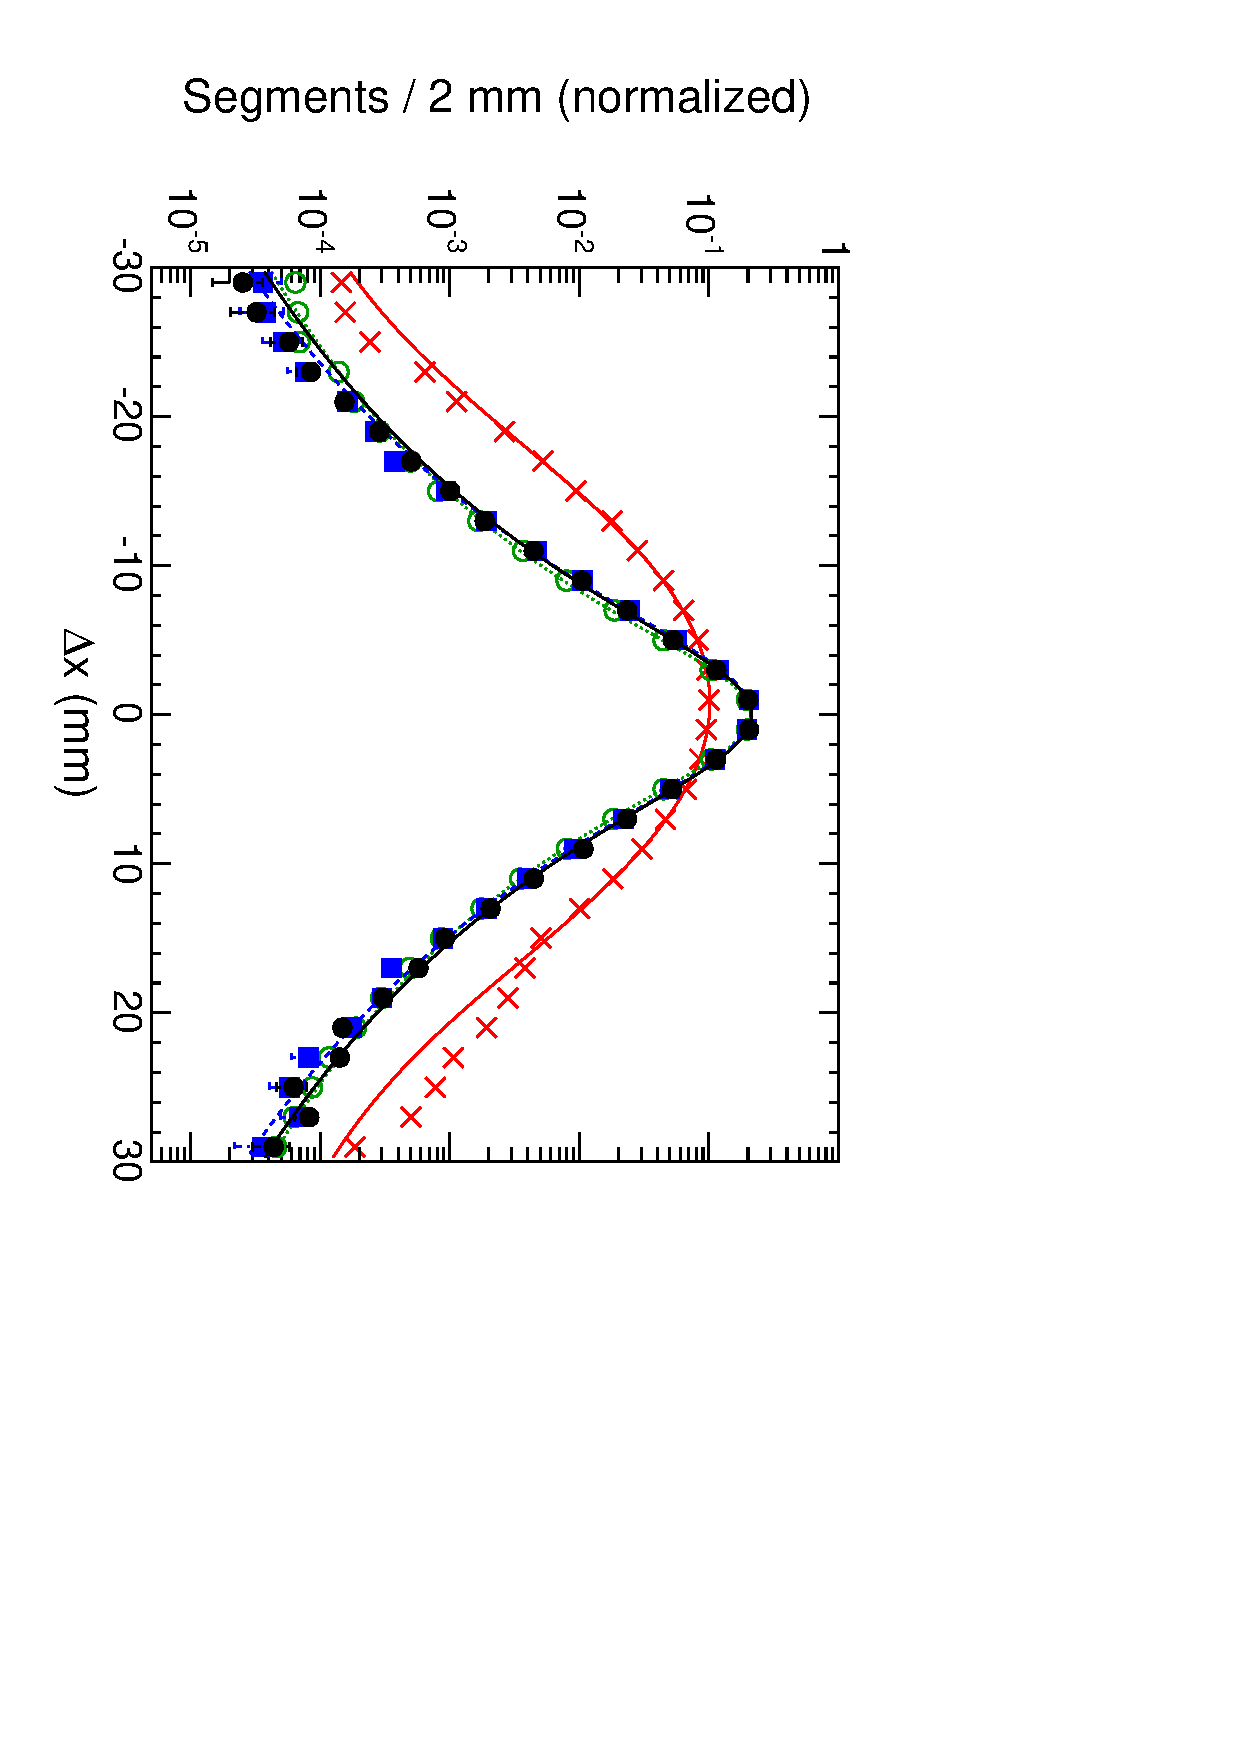
\includegraphics[width=0.45\linewidth]{plots/gma_hip_results/finalresiduals_alllogy_x.pdf}
\hfill 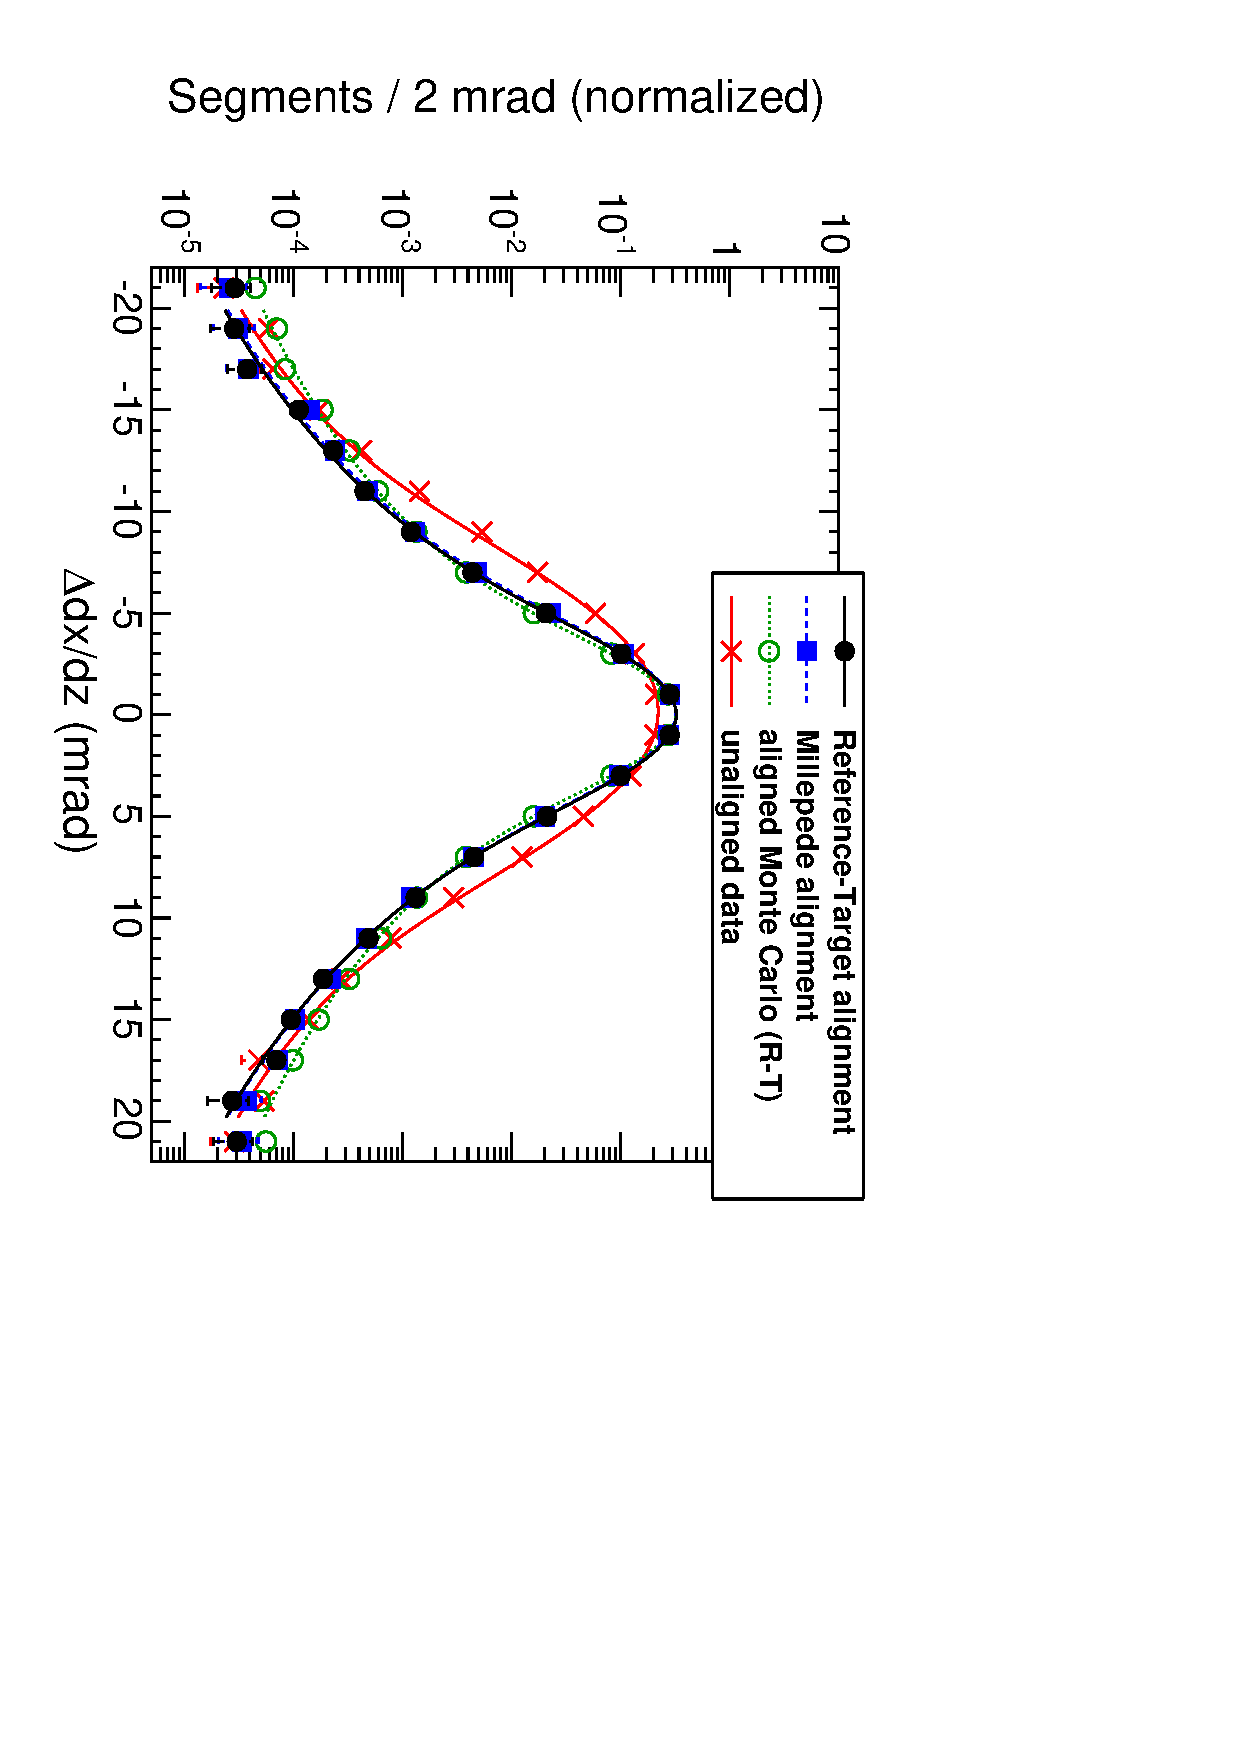
\includegraphics[width=0.45\linewidth]{plots/gma_hip_results/finalresiduals_alllogy_dxdz.pdf} \hfill \mbox{ }

\mbox{ } \hfill 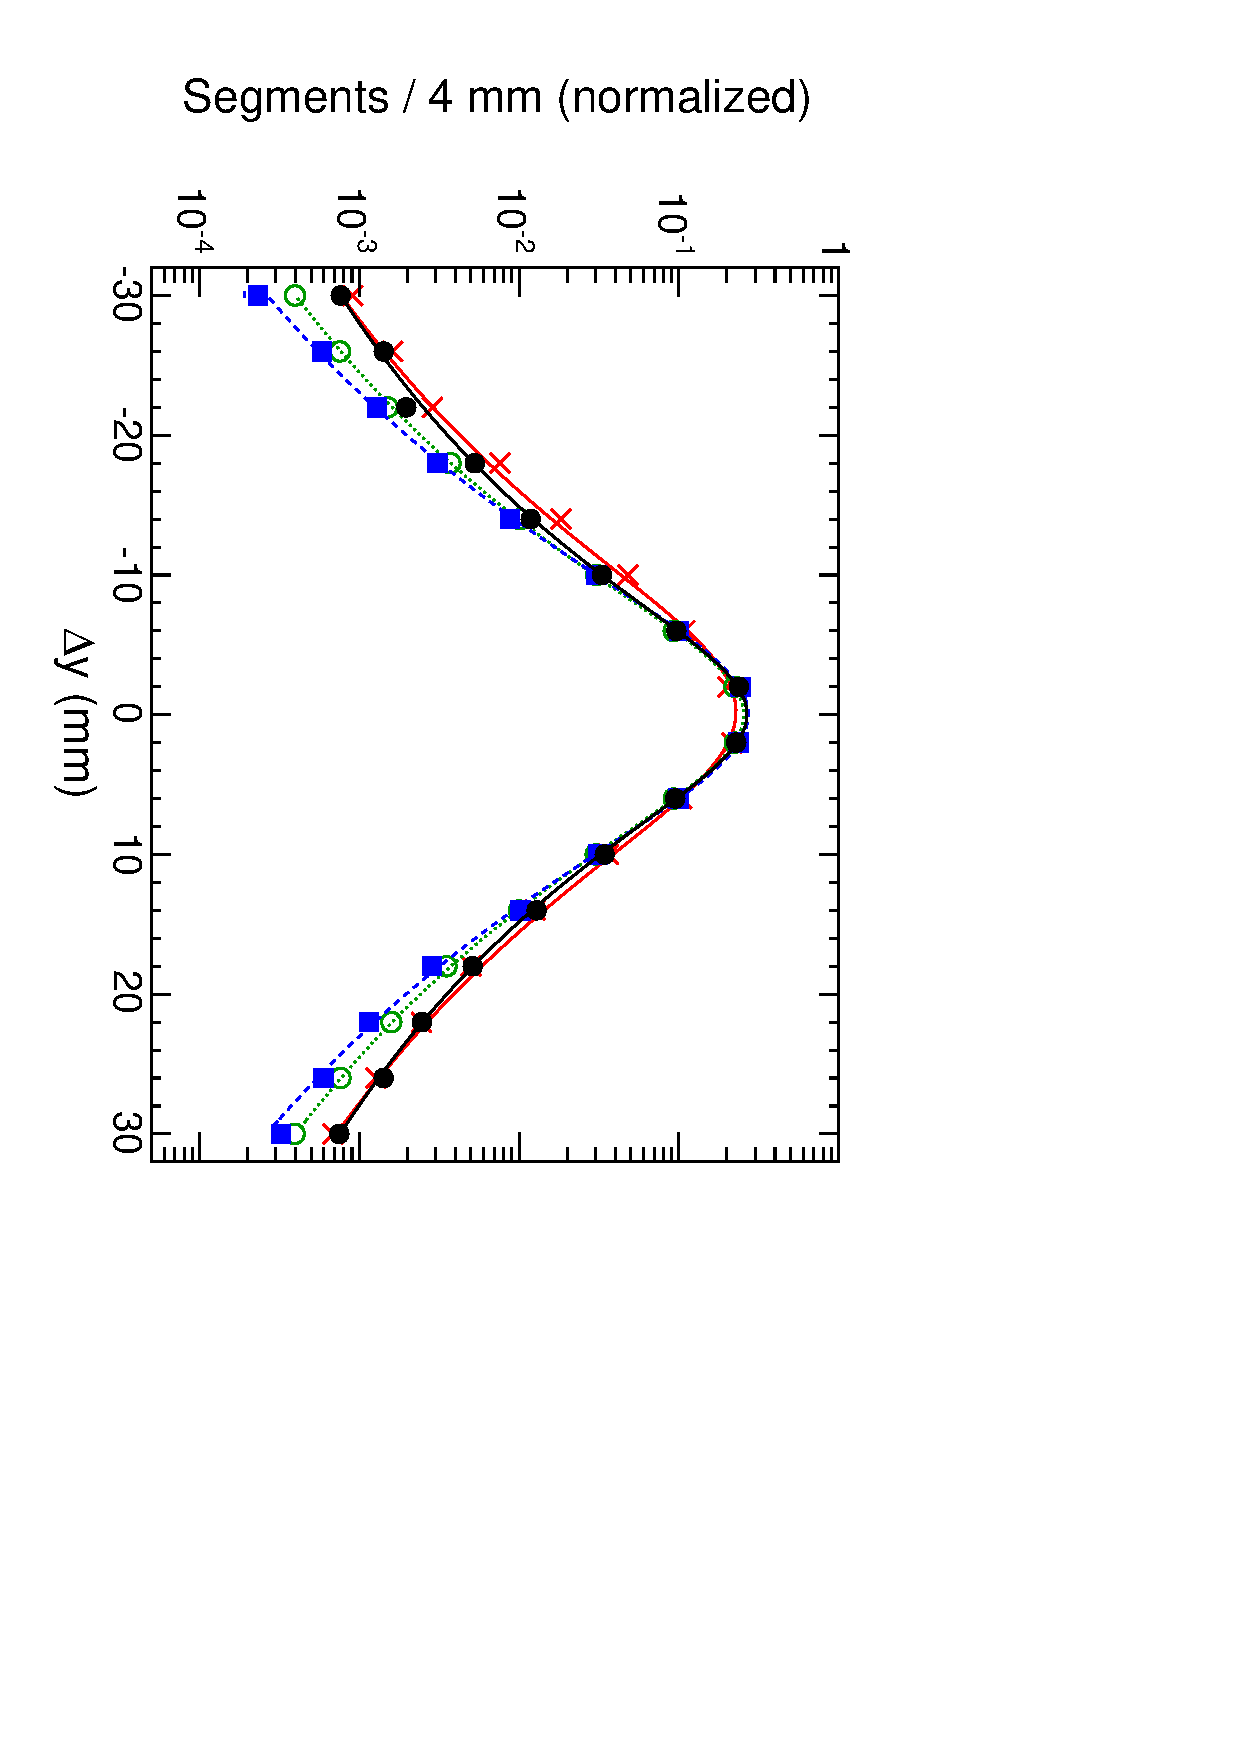
\includegraphics[width=0.45\linewidth]{plots/gma_hip_results/finalresiduals_alllogy_y.pdf}
\hfill 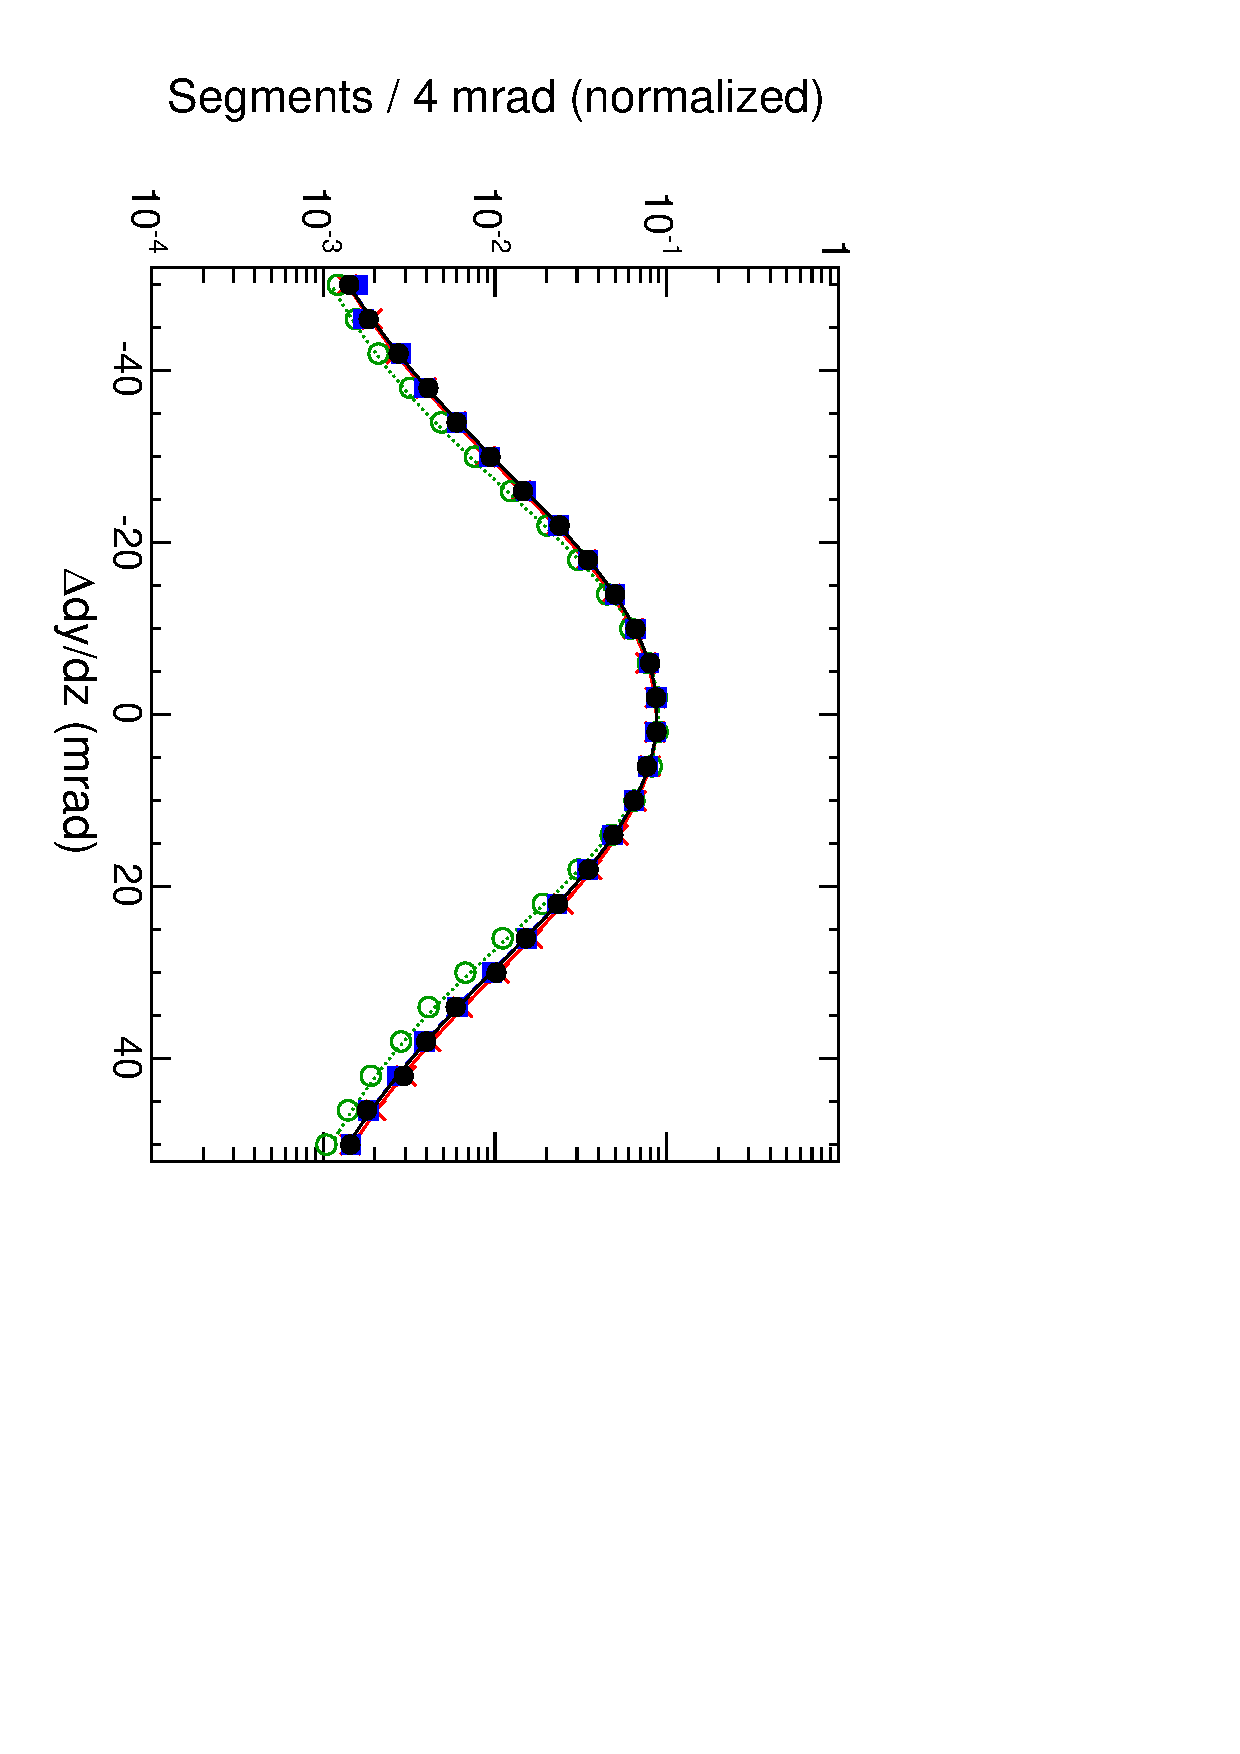
\includegraphics[width=0.45\linewidth]{plots/gma_hip_results/finalresiduals_alllogy_dydz.pdf} \hfill \mbox{ }
\caption{something \label{fig:residuals_all}}
\end{figure}

\begin{figure}
\mbox{ } \hfill 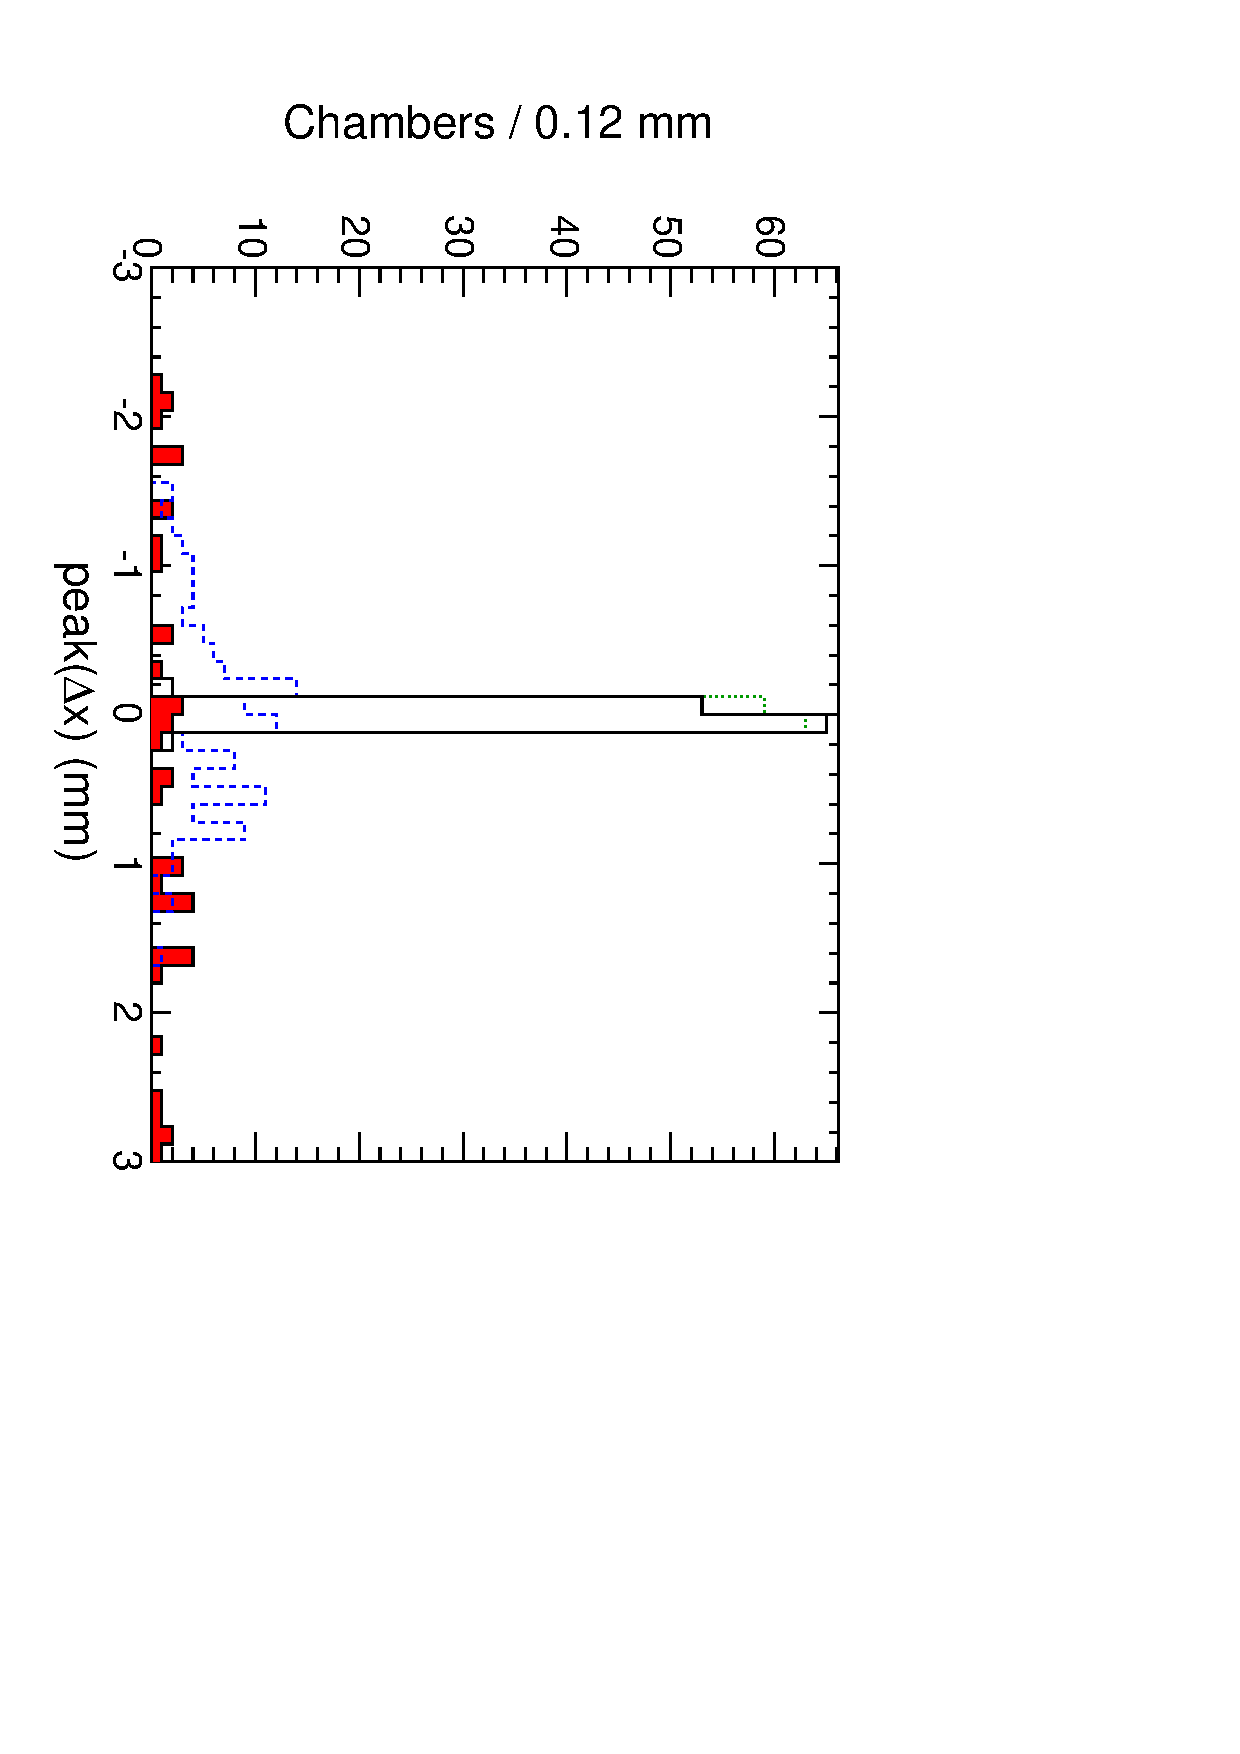
\includegraphics[width=0.45\linewidth]{plots/gma_hip_results/finalresiduals_peak_x.pdf}
\hfill 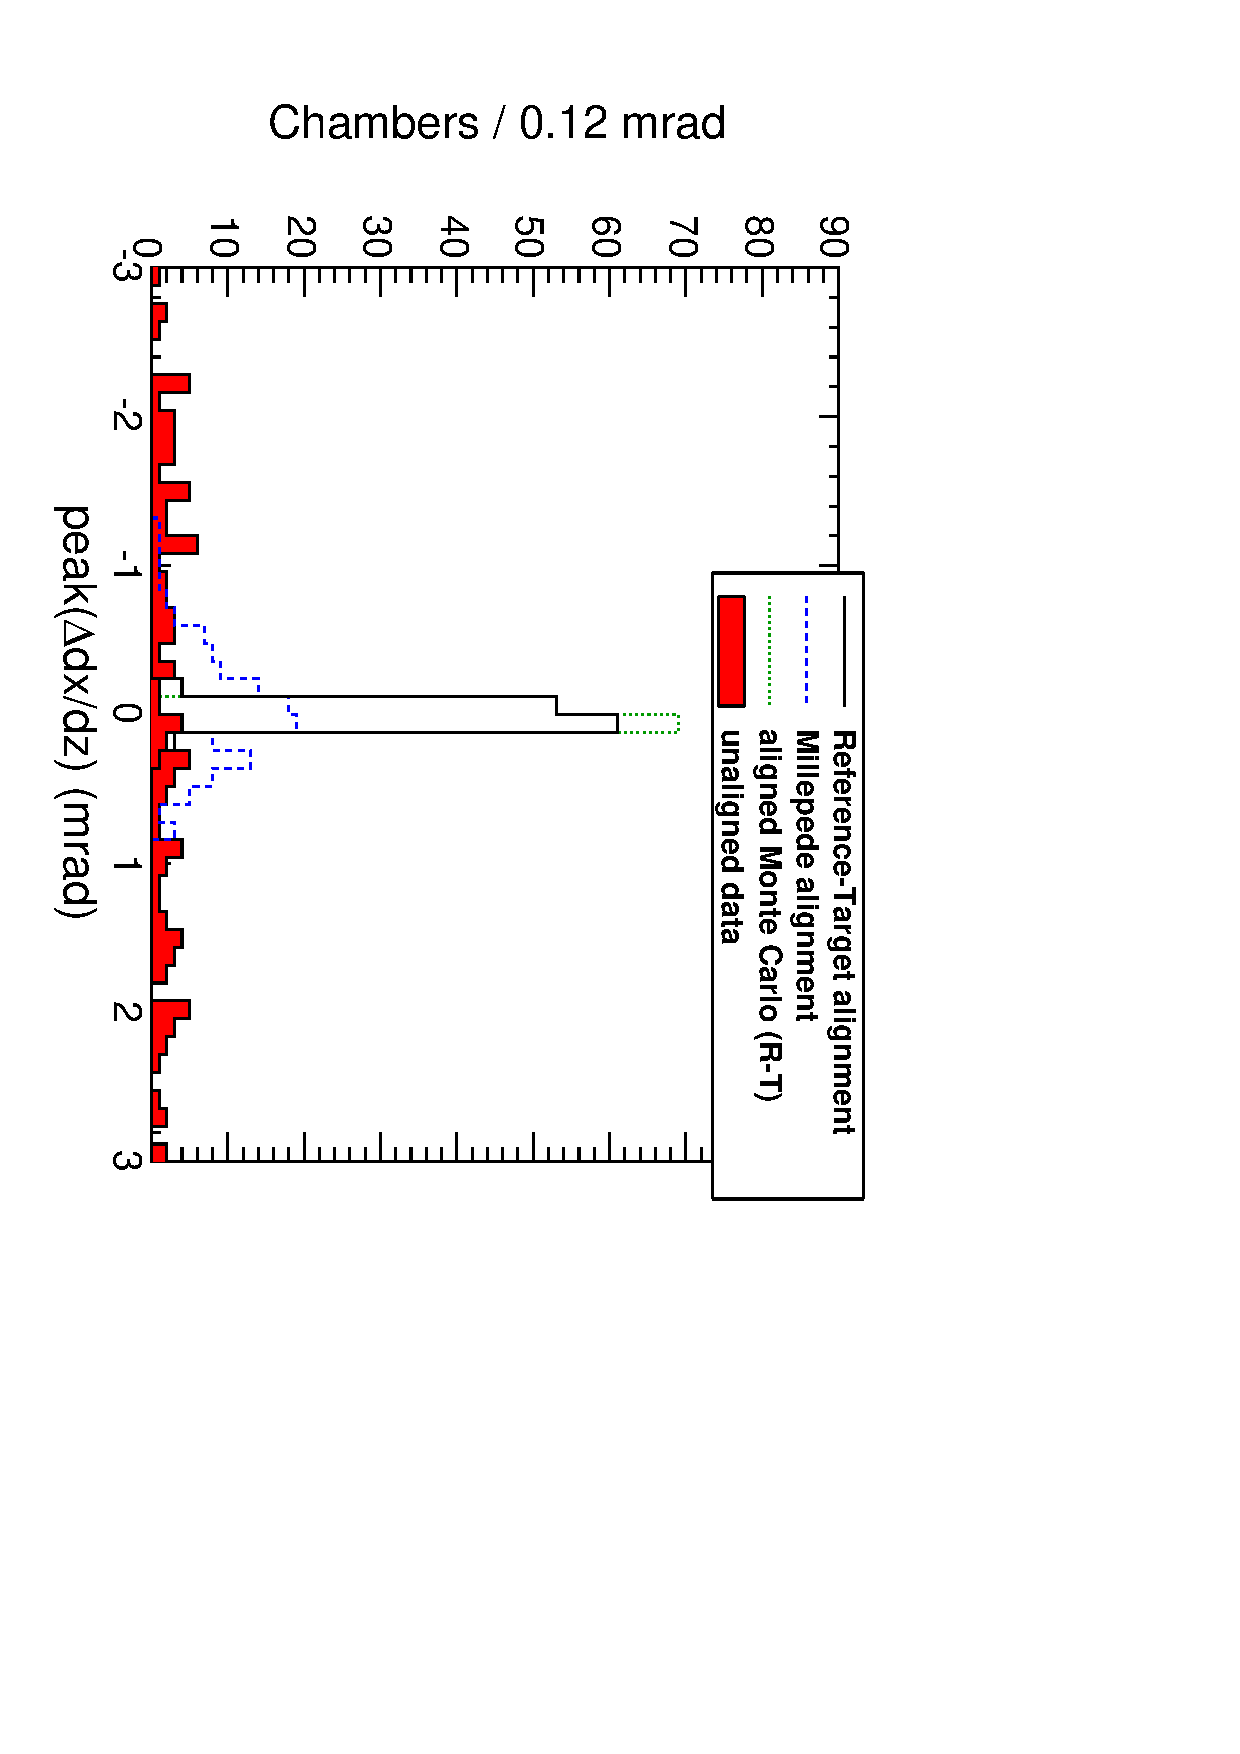
\includegraphics[width=0.45\linewidth]{plots/gma_hip_results/finalresiduals_peak_dxdz.pdf} \hfill \mbox{ }

\mbox{ } \hfill 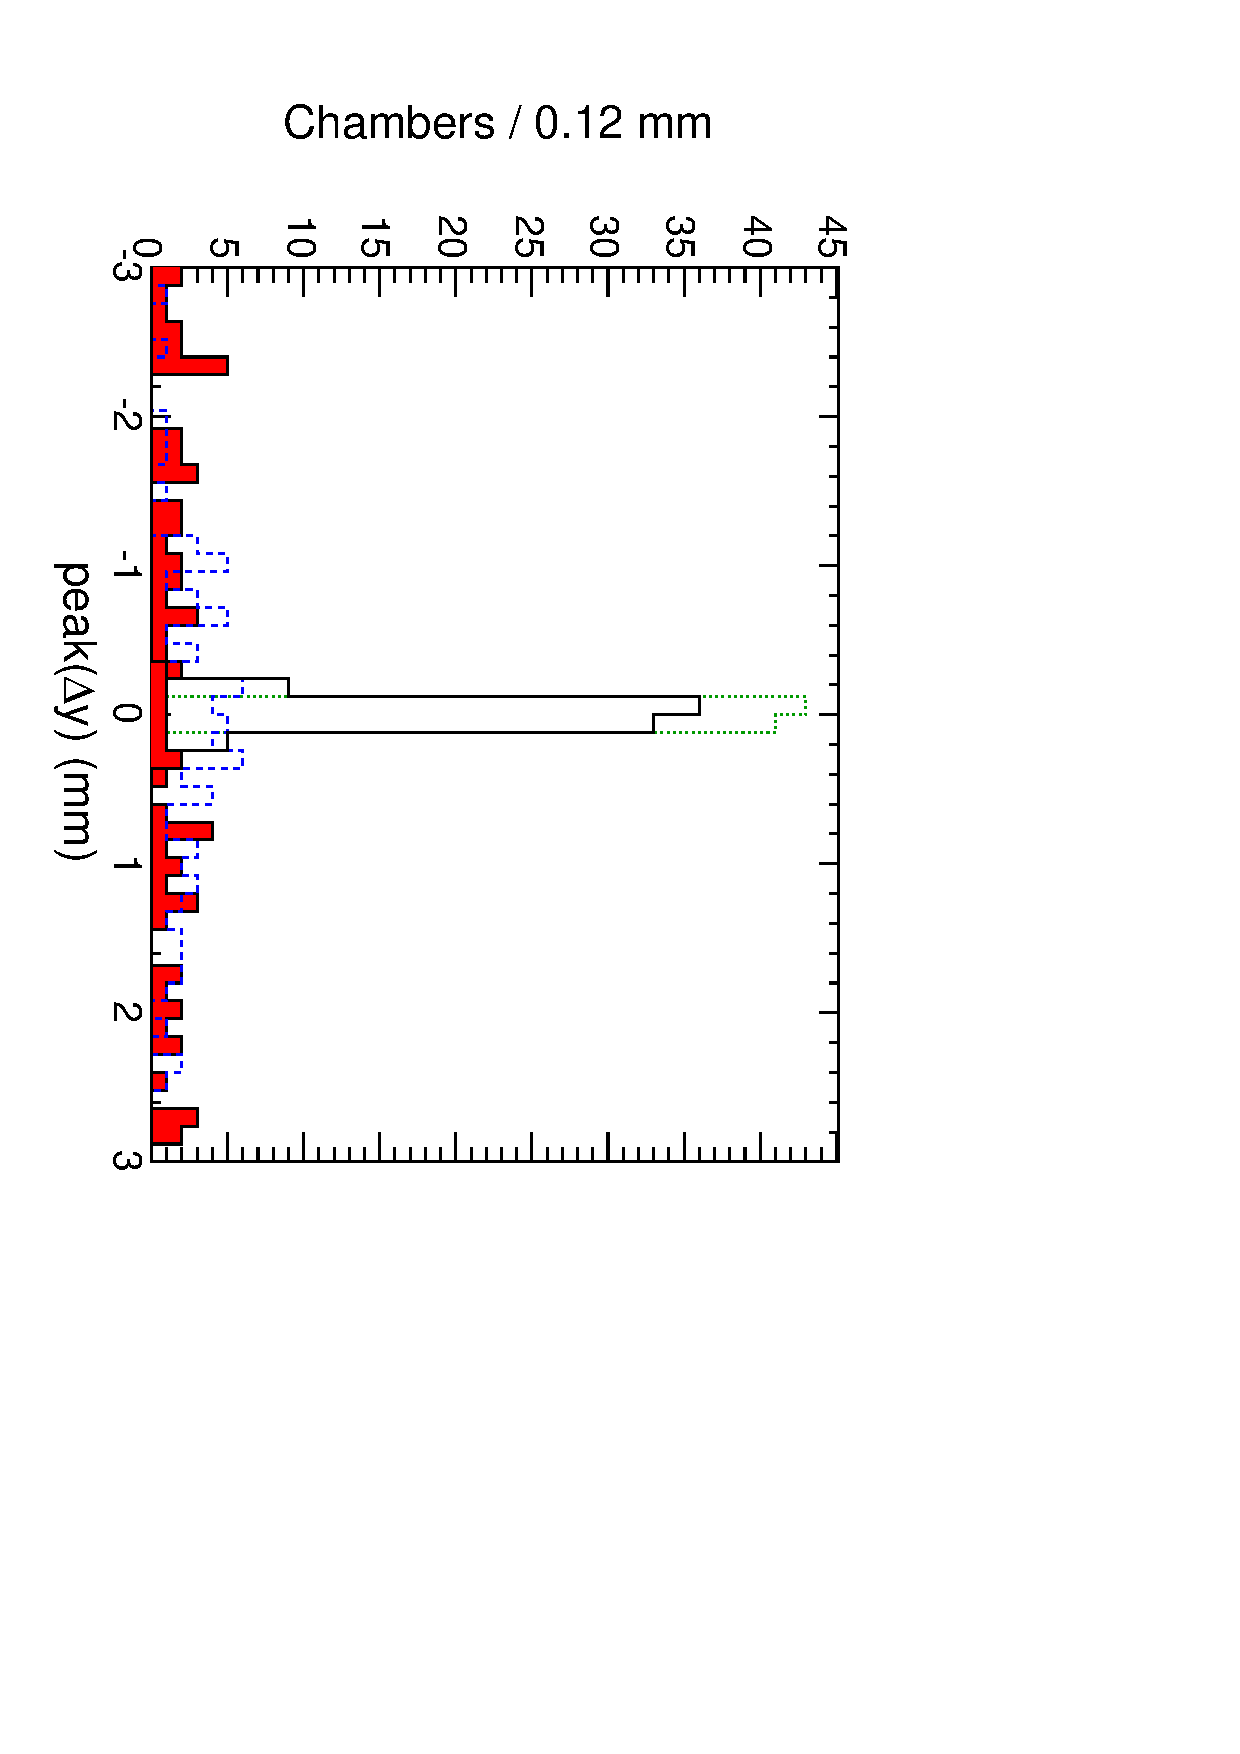
\includegraphics[width=0.45\linewidth]{plots/gma_hip_results/finalresiduals_peak_y.pdf}
\hfill 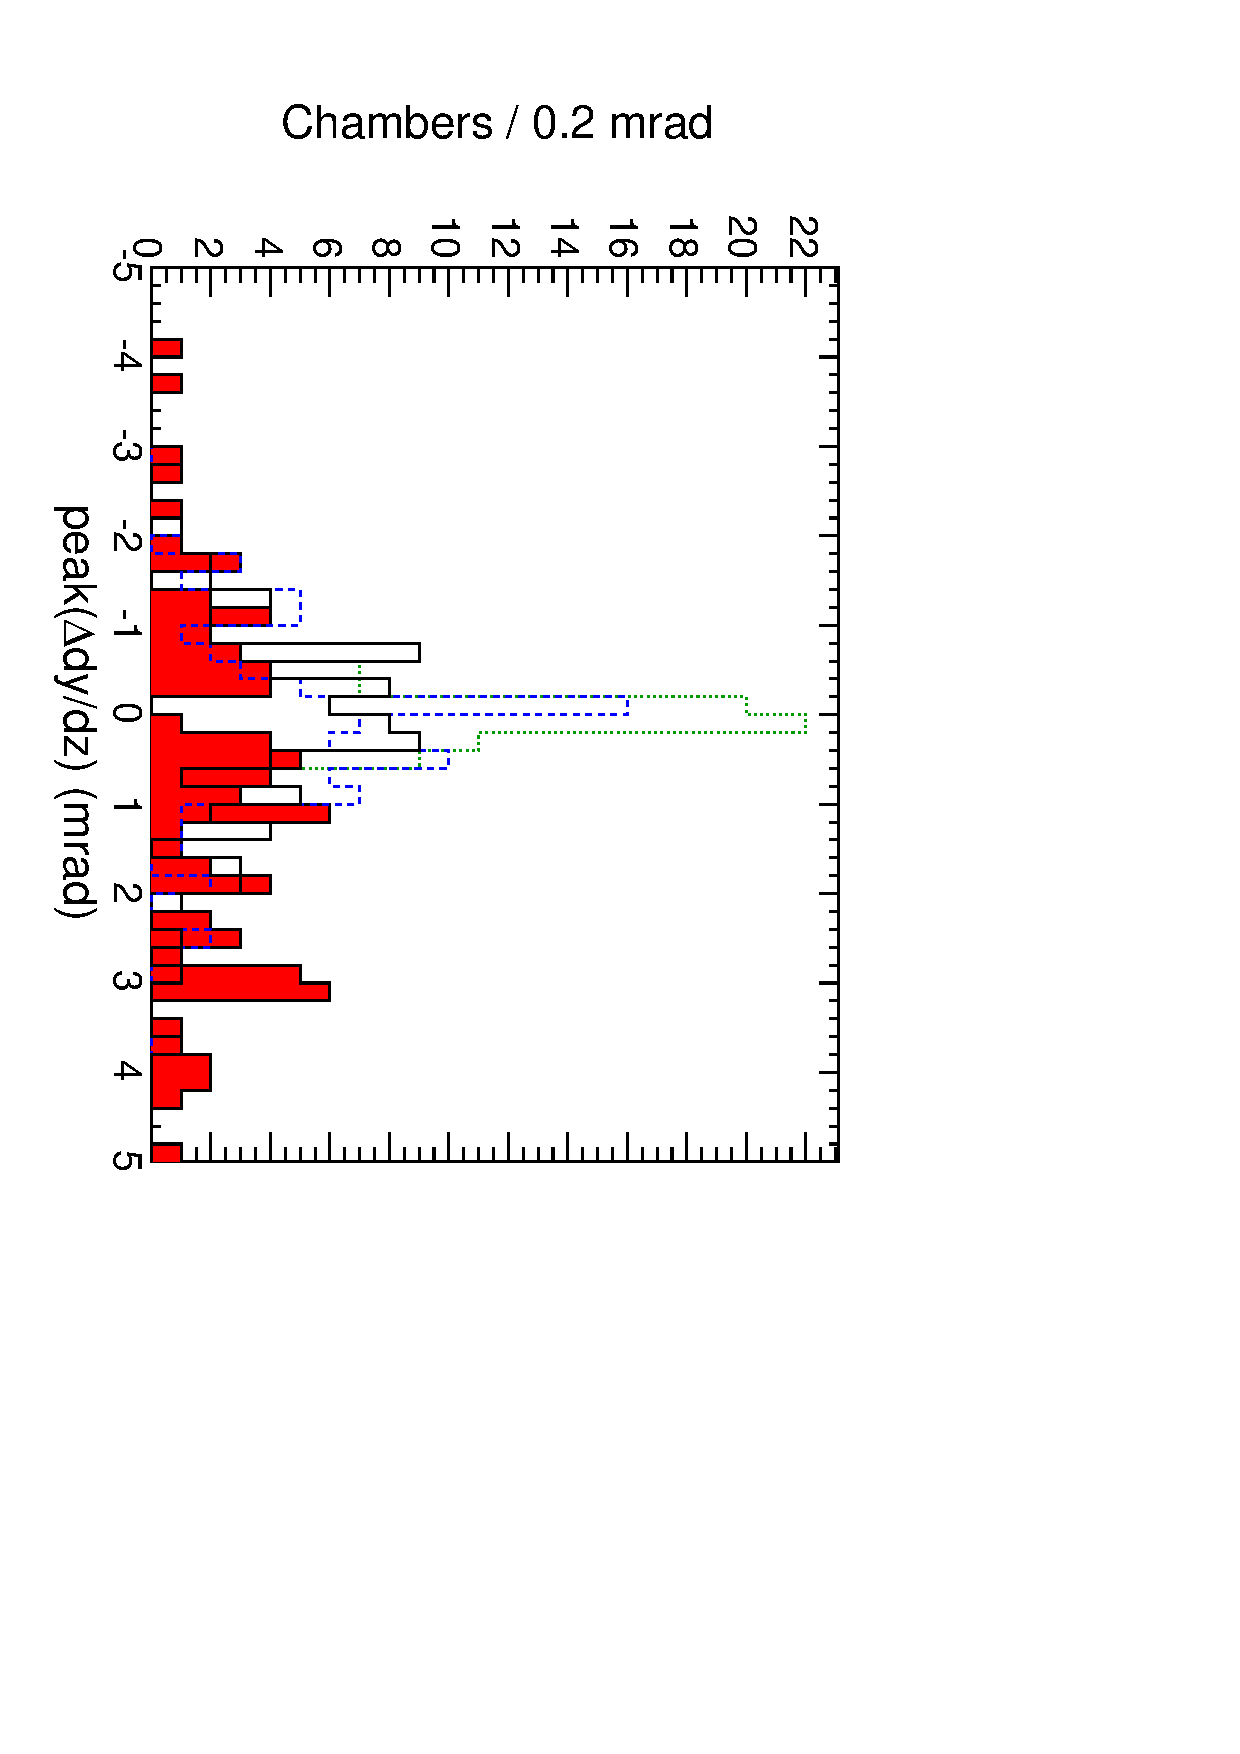
\includegraphics[width=0.45\linewidth]{plots/gma_hip_results/finalresiduals_peak_dydz.pdf} \hfill \mbox{ }
\caption{something \label{fig:residuals_peak}}
\end{figure}

\begin{figure}
\mbox{ } \hfill 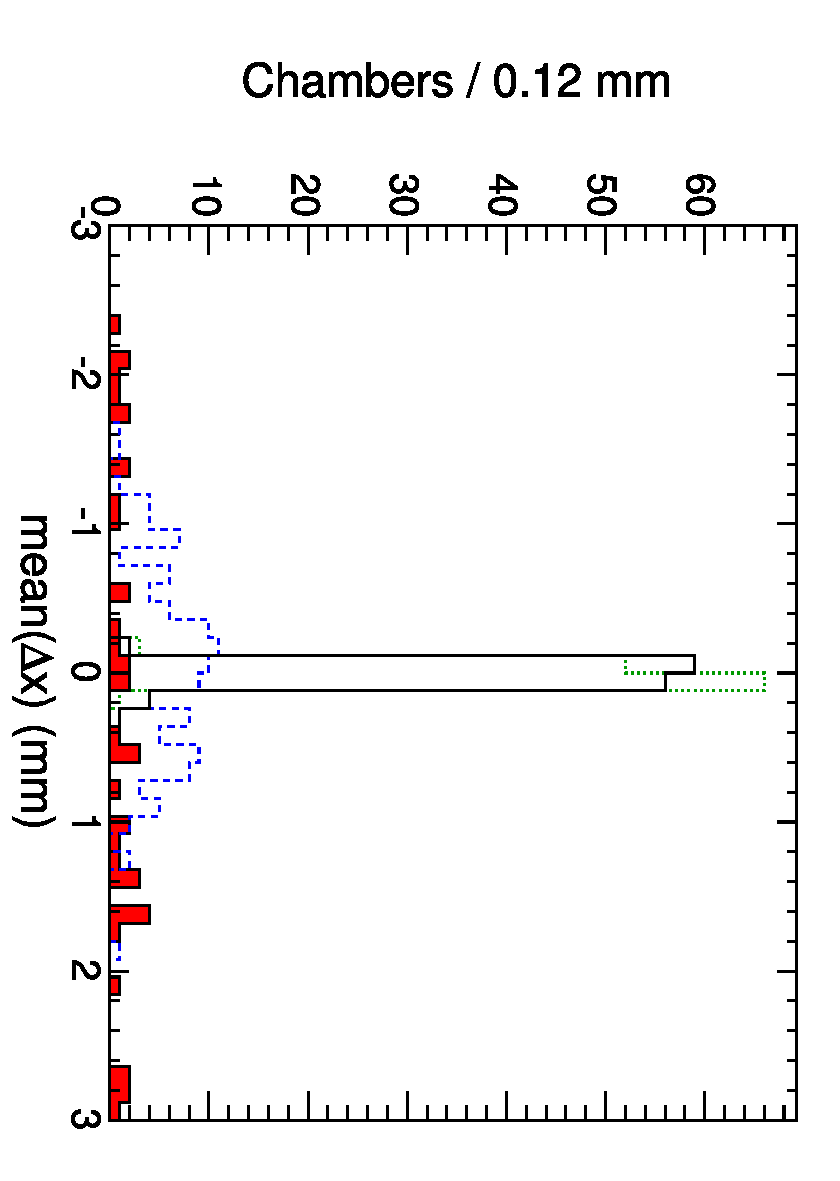
\includegraphics[width=0.45\linewidth]{plots/gma_hip_results/finalresiduals_mean_x.pdf}
\hfill 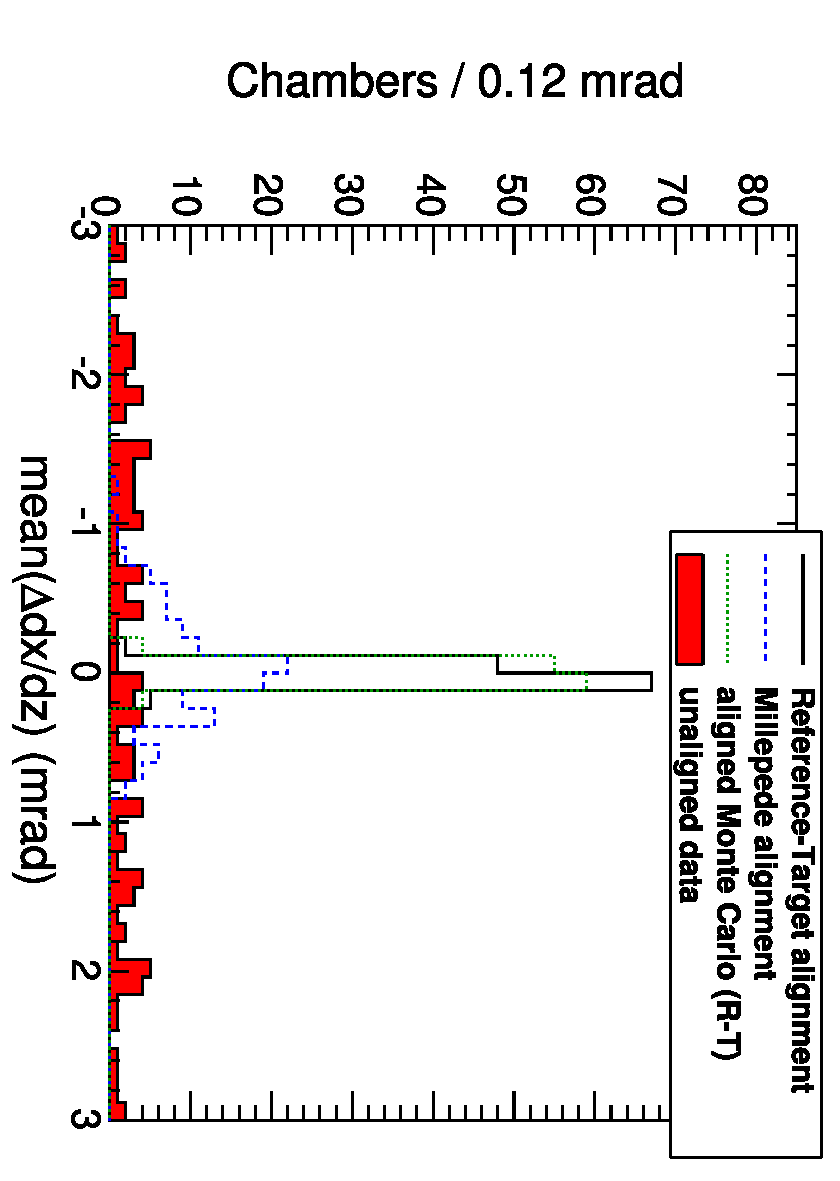
\includegraphics[width=0.45\linewidth]{plots/gma_hip_results/finalresiduals_mean_dxdz.pdf} \hfill \mbox{ }

\mbox{ } \hfill 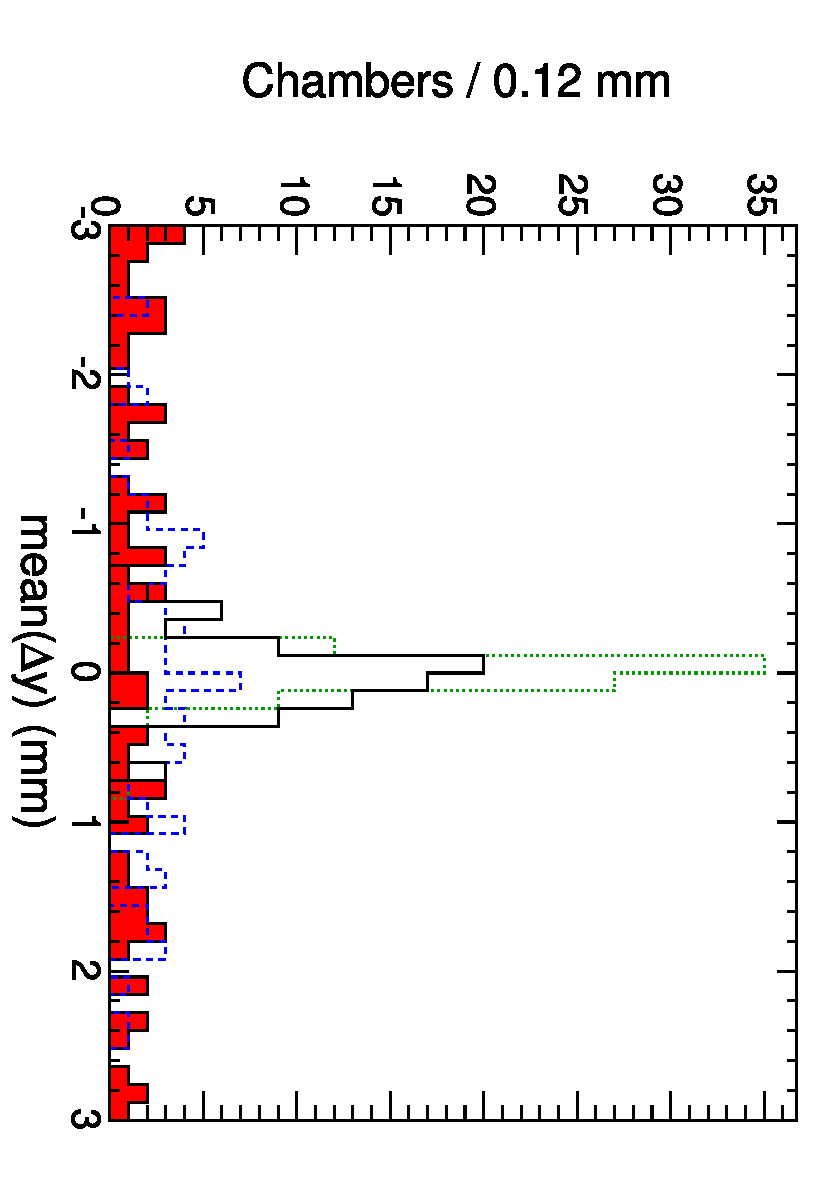
\includegraphics[width=0.45\linewidth]{plots/gma_hip_results/finalresiduals_mean_y.pdf}
\hfill 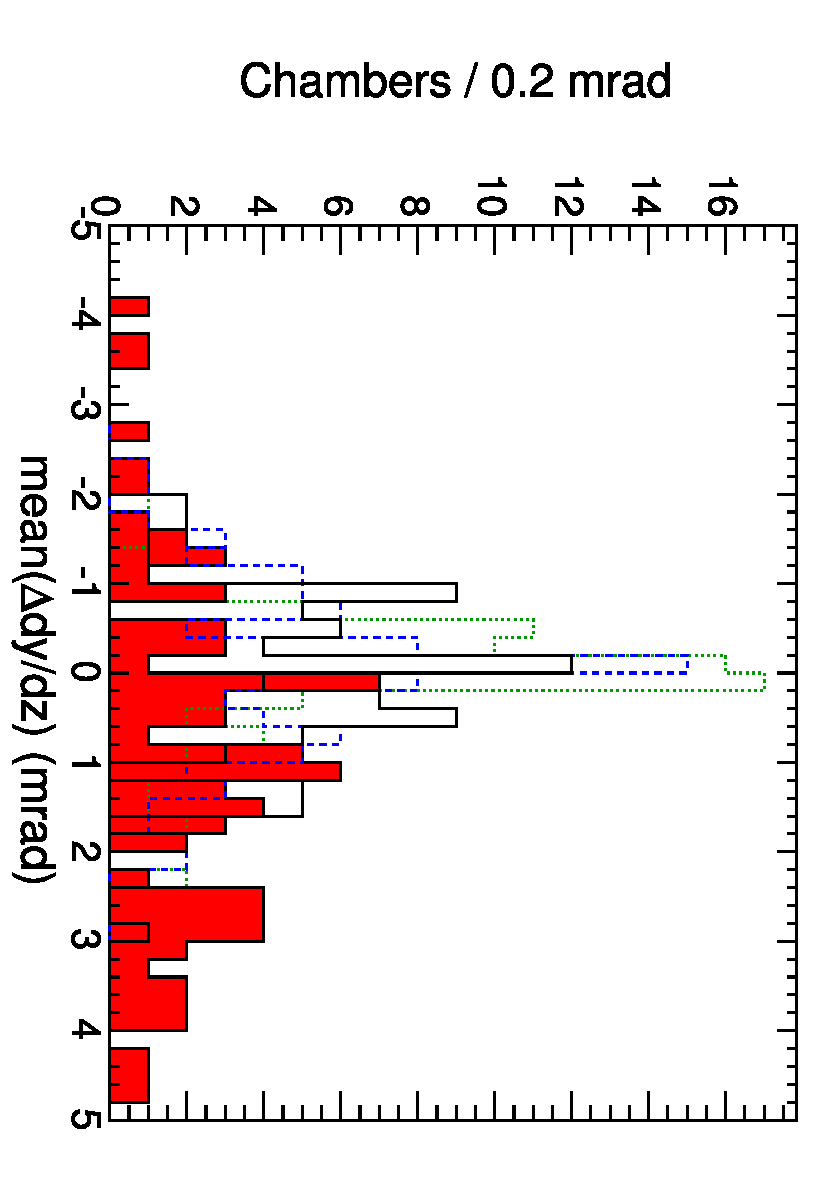
\includegraphics[width=0.45\linewidth]{plots/gma_hip_results/finalresiduals_mean_dydz.pdf} \hfill \mbox{ }
\caption{alterative for Figure~\ref{fig:residuals_peak} \label{fig:residuals_mean}}
\end{figure}

\begin{figure}
\begin{center}
%% 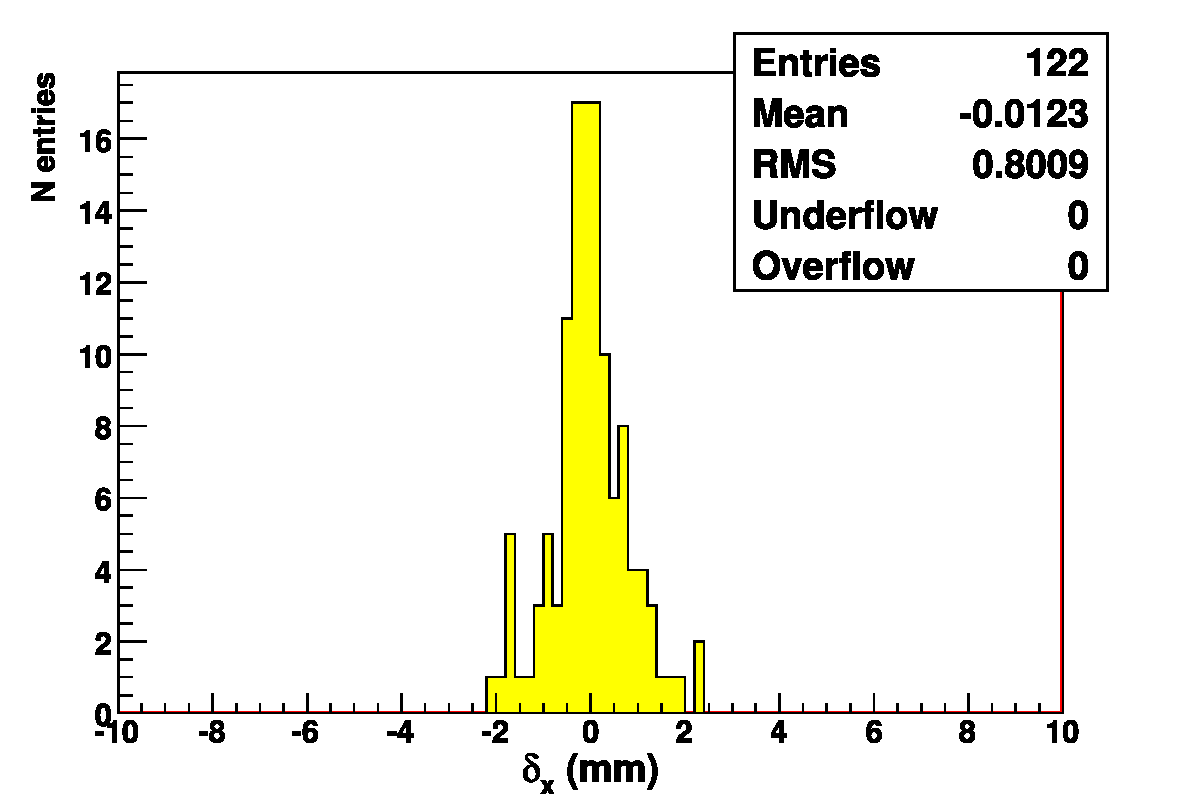
\includegraphics[width=0.32\linewidth]{plots/gma_hip_results/delta_xComparison.pdf}
%% 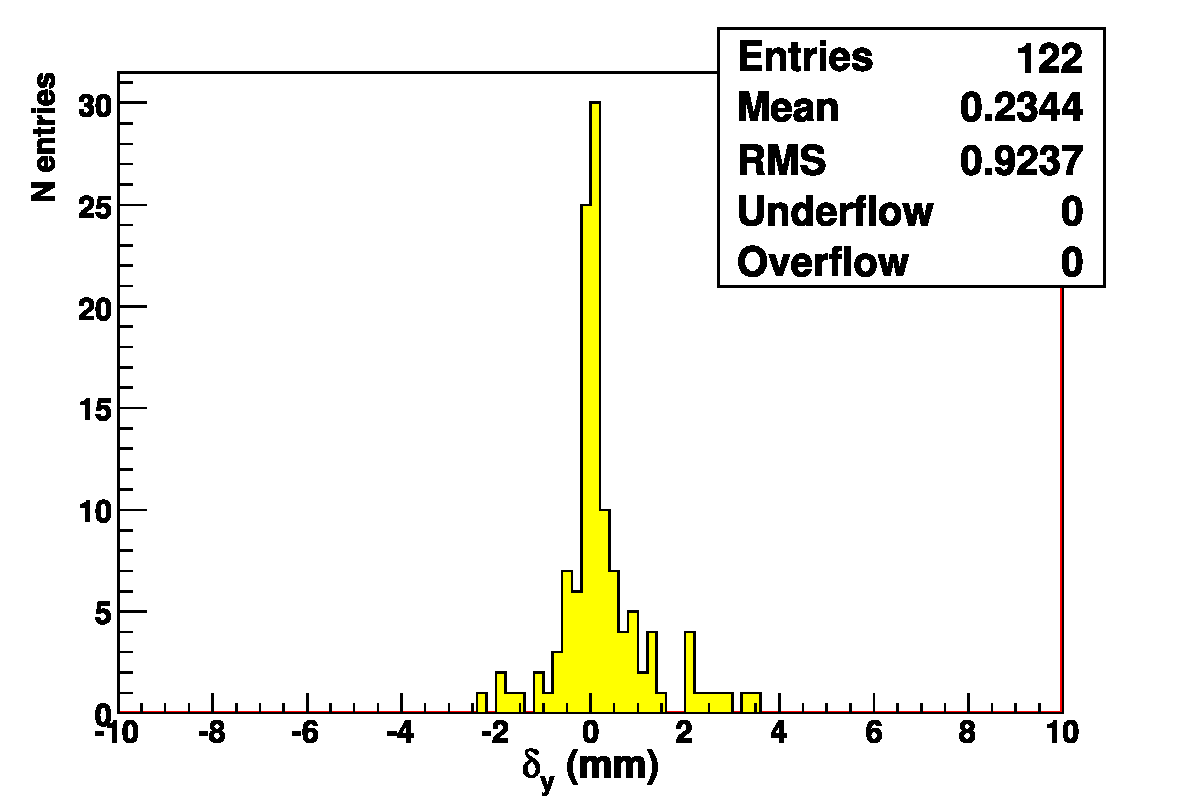
\includegraphics[width=0.32\linewidth]{plots/gma_hip_results/delta_yComparison.pdf}
%% 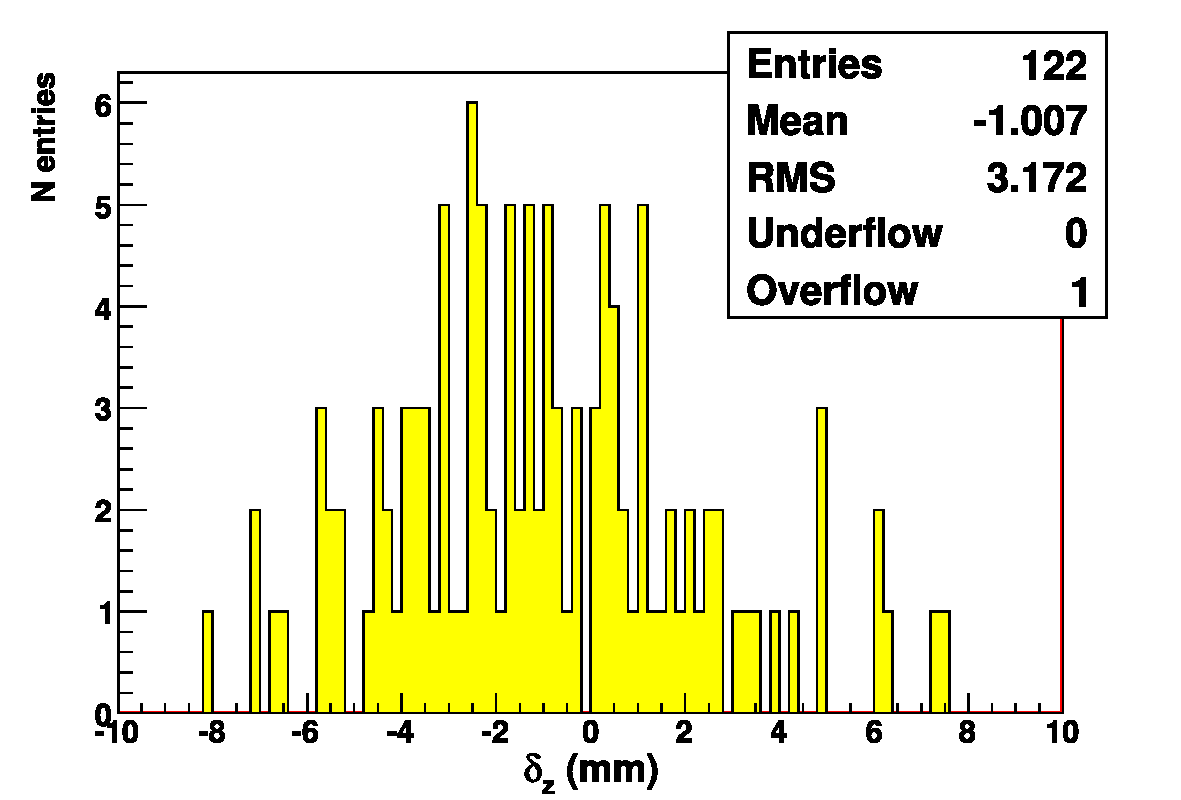
\includegraphics[width=0.32\linewidth]{plots/gma_hip_results/delta_zComparison.pdf}

%% 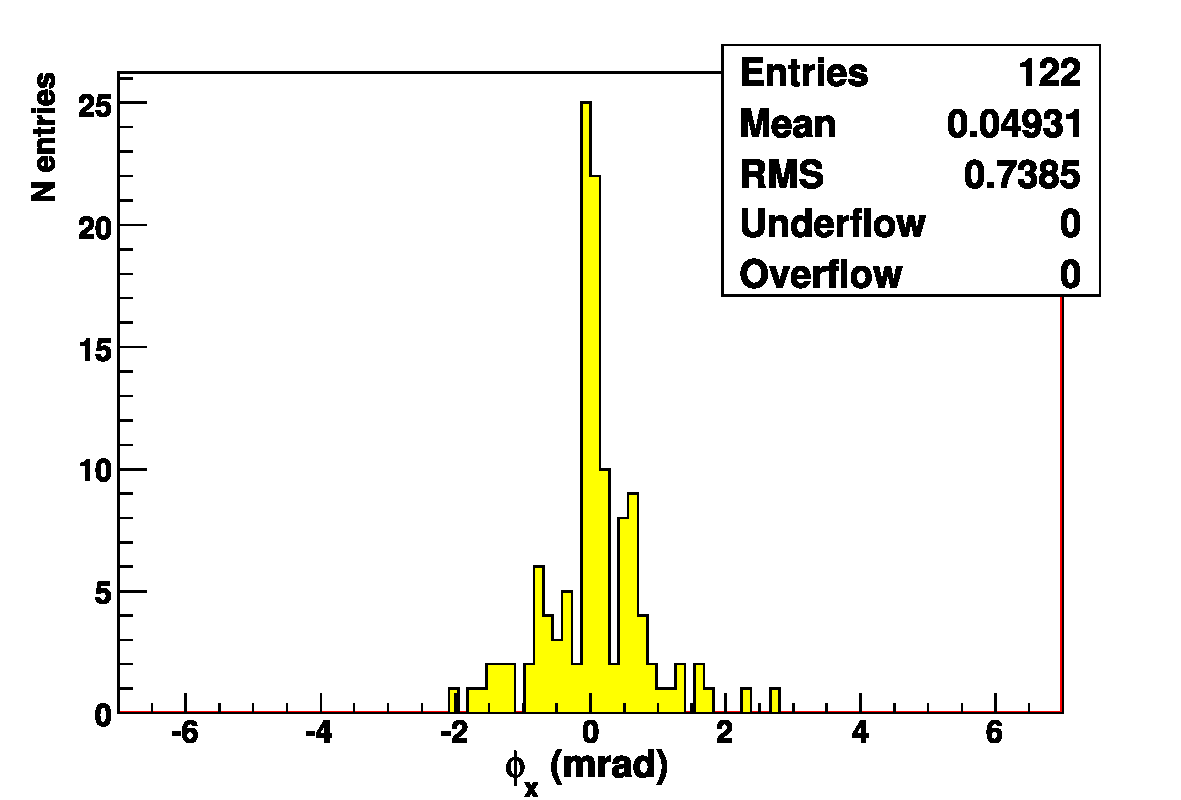
\includegraphics[width=0.32\linewidth]{plots/gma_hip_results/phixComparison.pdf}
%% 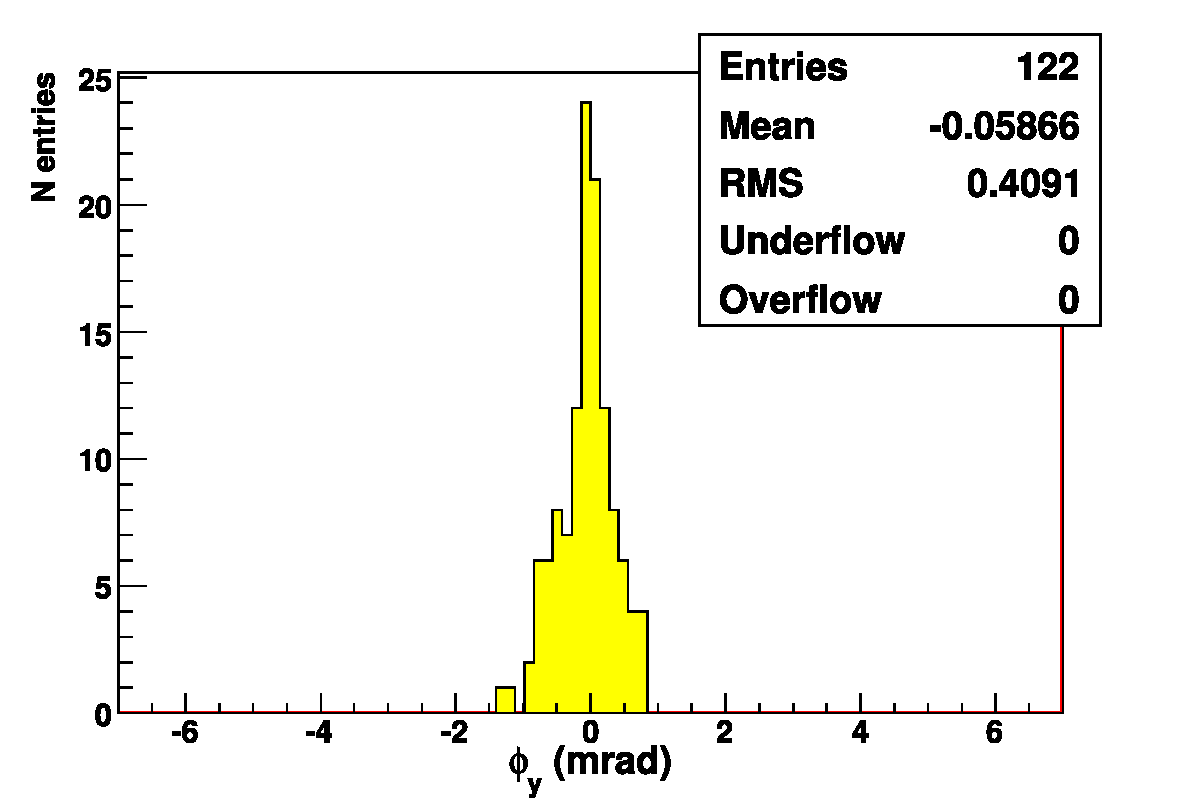
\includegraphics[width=0.32\linewidth]{plots/gma_hip_results/phiyComparison.pdf}
%% 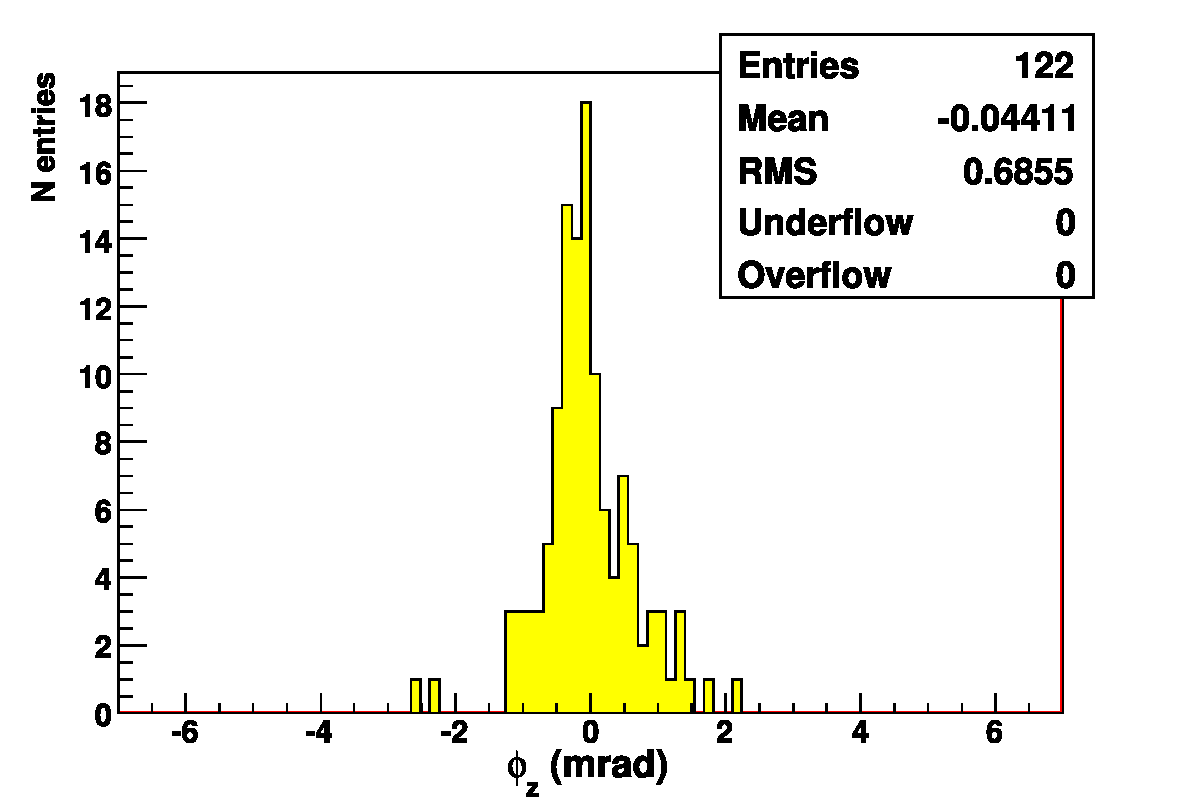
\includegraphics[width=0.32\linewidth]{plots/gma_hip_results/phizComparison.pdf}

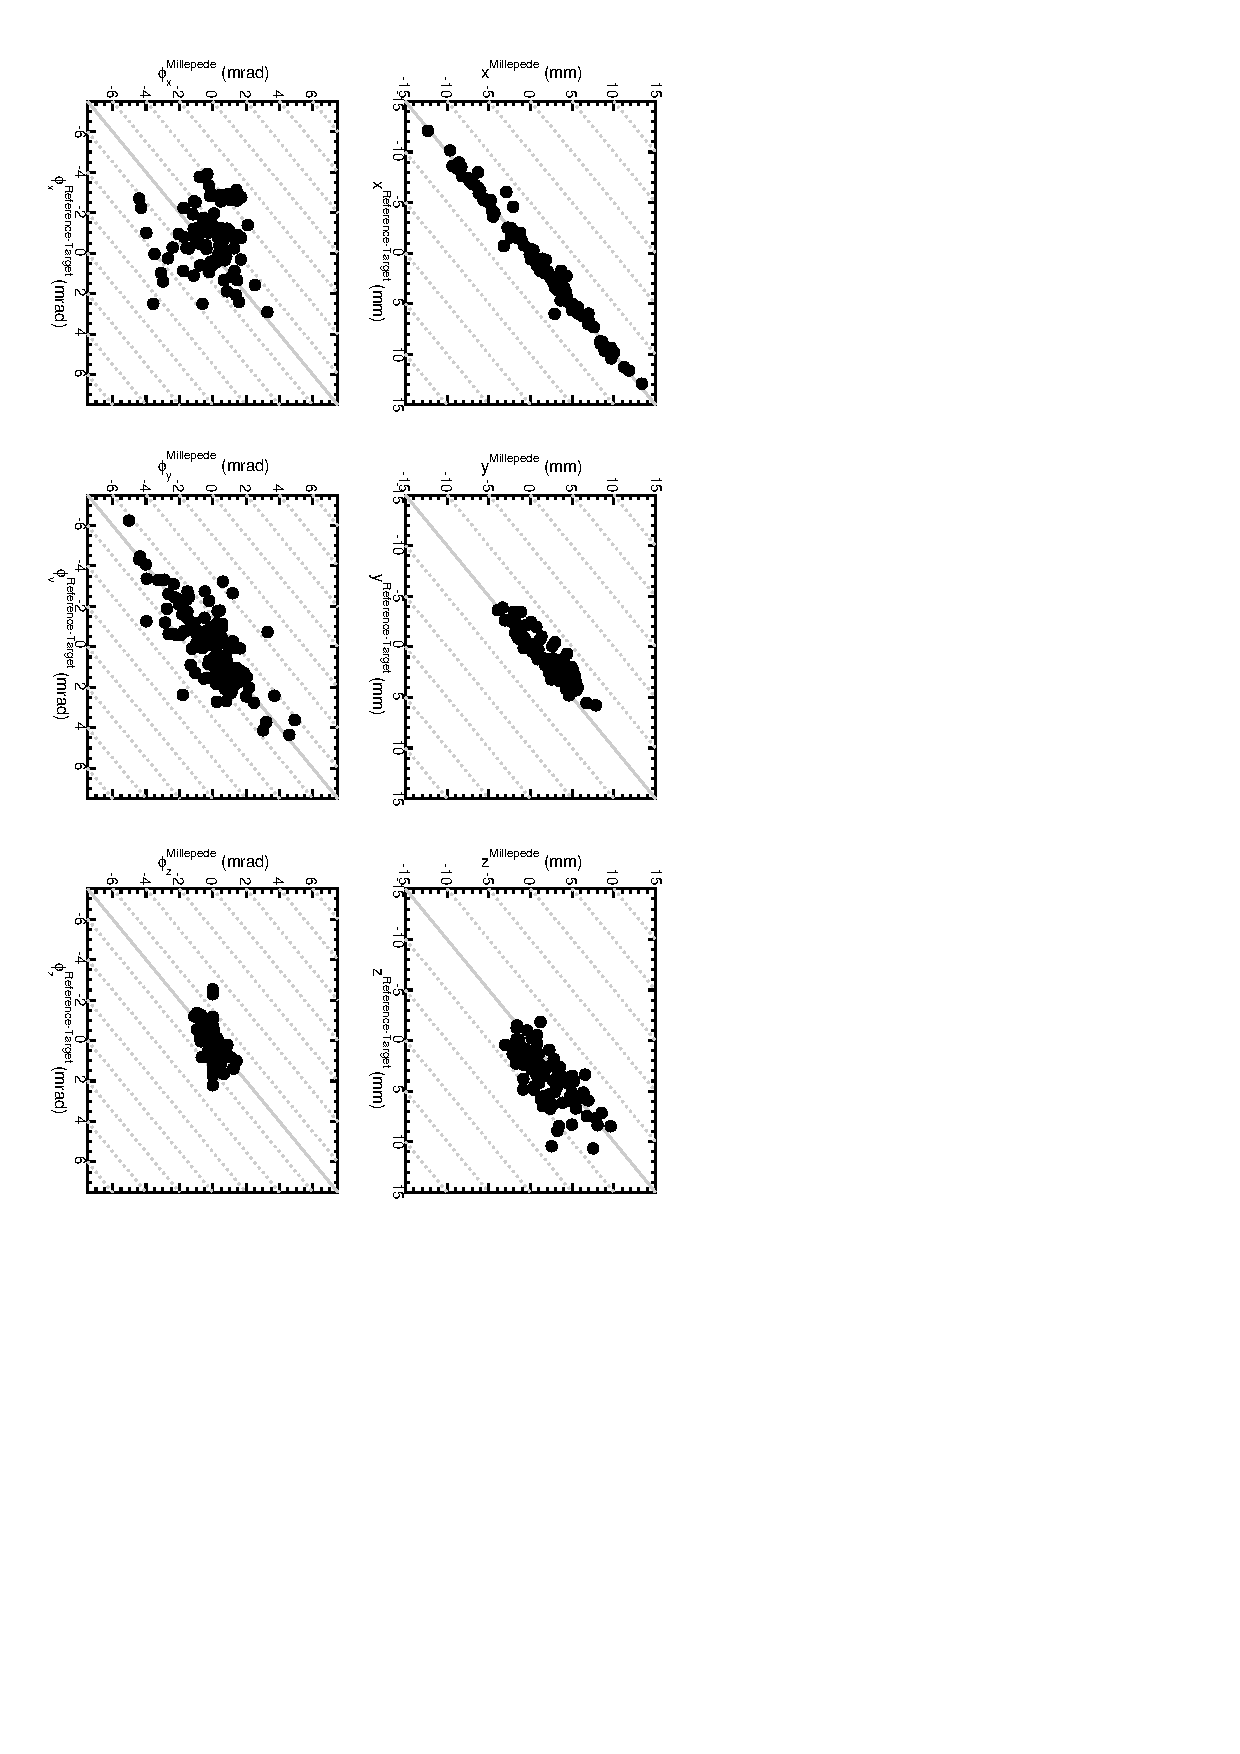
\includegraphics[height=\linewidth, angle=90]{plots/gma_hip_results/MP-V4_vs_HIP-V4.pdf}
\end{center}
\caption{Alignment corrections determined by the HIP and Millepede algorithms. (Only aligned chambers are shown.)\label{fig:sidebyside}}
\end{figure}

Local alignment measurements to test consistency between global data
and local data (3) were derived by extrapolating linear track segments
from one chamber to the next (in the same sector, neighboring
stations).  This verification procedure introduces information not
used in the alignment itself, namely the higher precision with which
tracks can be propagated over a short distance (1~meter) than a long
distance (3--6~meters).

For this diagnostic, tracks were selected with $p_T > 50$~GeV and a
correction was applied to cancel the effect of the magnetic field by
taking advantage of the fact that positively- and negatively-charged
tracks are pushed in opposite directions.
%% Figure~\ref{fig:valid_DTconsts} shows the level of agreement in $x$
%% position and $\frac{dx}{dz}$ angle between segments in neighboring
%% stations for each sector in wheel~0.
To compare the initial state with the results of each algorithm in all
station-pairs, sectors, and wheels, we filled histograms with the
fitted Gaussian peak of each comparison, shown in
Figure~\ref{fig:valid_NOMvsMPvsHIP}.  Though the global alignment
algorithms changed the positions of chambers by 2.5~mm in the local
$x$ direction (RMS in Figure~\ref{fig:sidebyside}), local differences
in $x$ are typically 0.7~mm (RMS of $x$ in
Figure~\ref{fig:valid_NOMvsMPvsHIP} for stations 1--3), and though
global algorithms changed $\phi_y$ by 1.5~mrad, local differences are
typically 0.6~mrad.  As expected, the chambers which are closest to
the tracker are the most precisely aligned.

%% \begin{figure}
%%   \centering
%%   \subfigure[Average $x$ difference between stations]{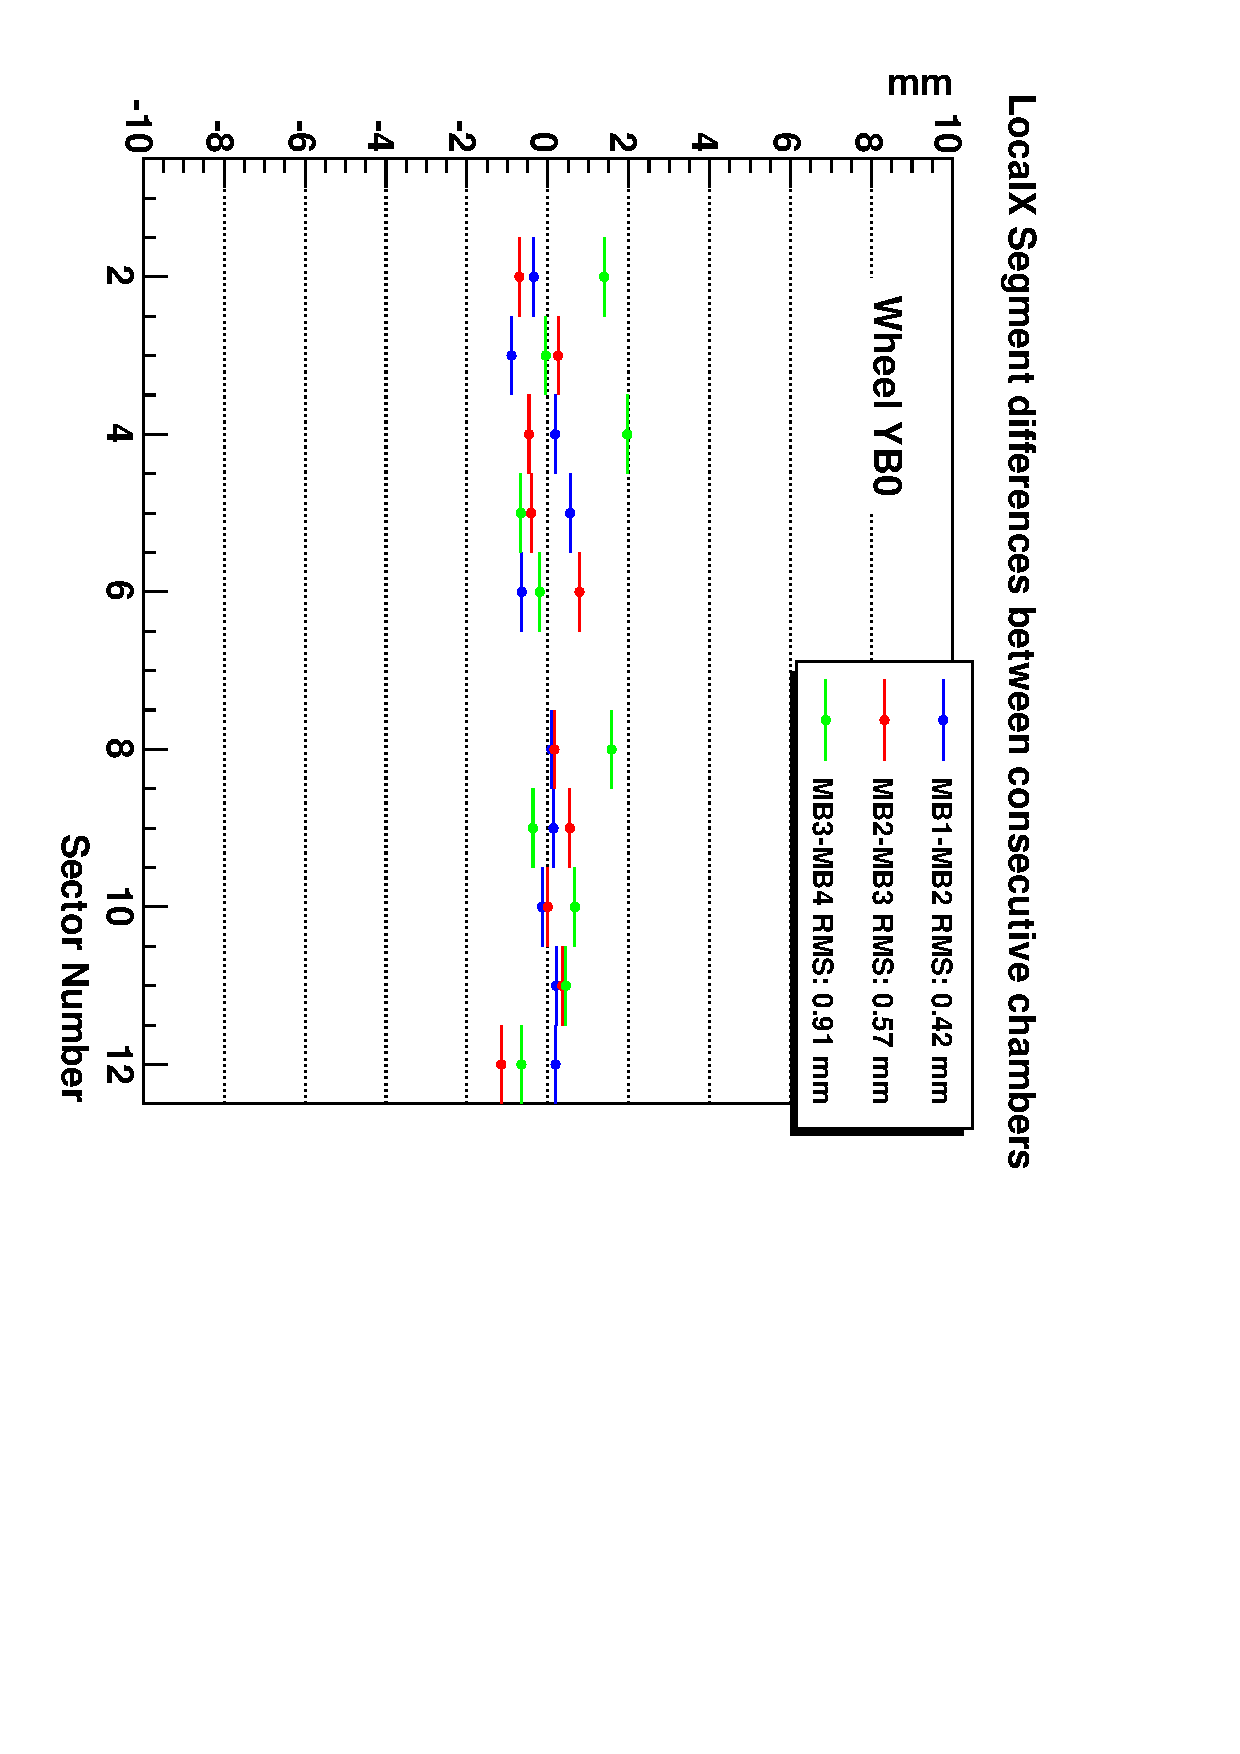
\includegraphics[width=0.4\textwidth, angle=90]{plots/validation/aligVal_08June09_LocalX_YB0.pdf}}
%%   \subfigure[Average $\frac{dx}{dz}$ difference between stations]{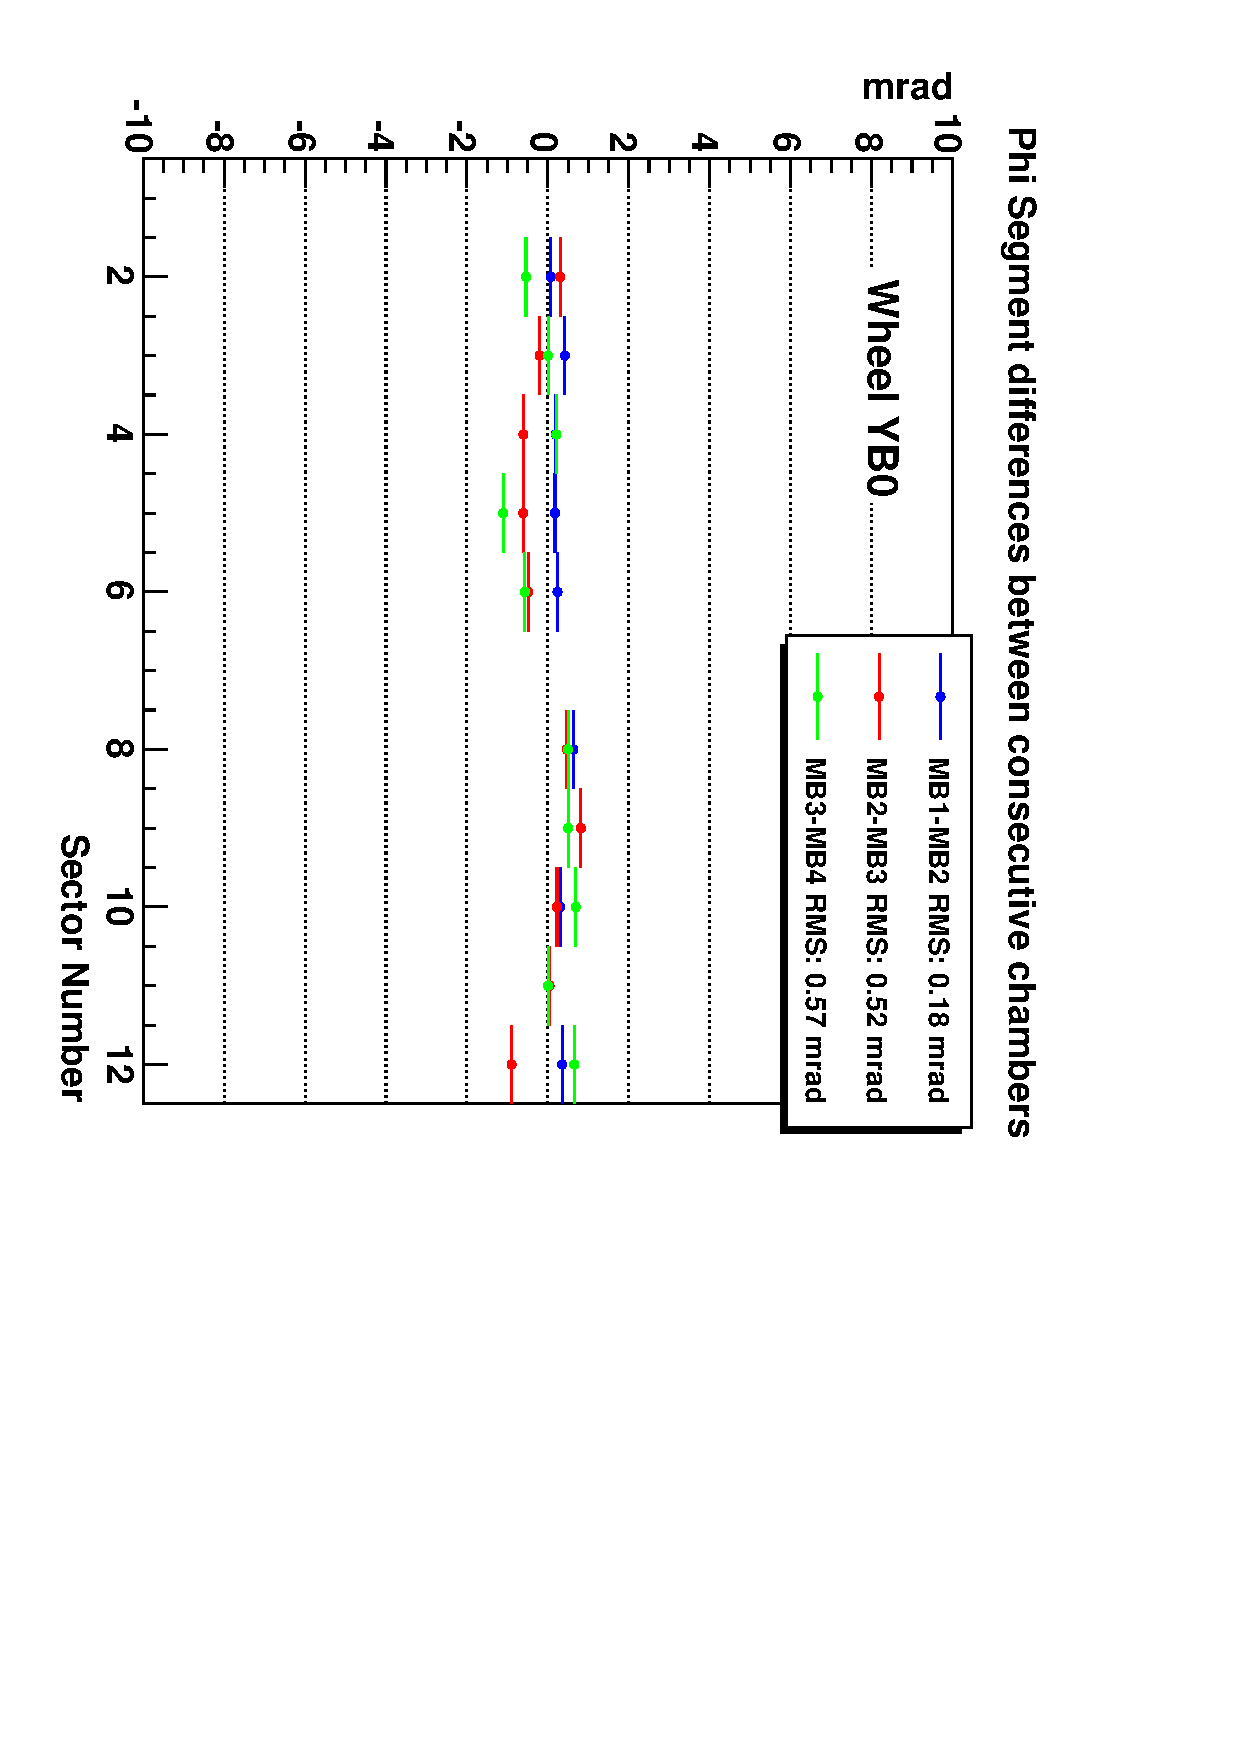
\includegraphics[width=0.4\textwidth, angle=90]{plots/validation/aligVal_08June09_Phi_YB0.pdf}}
%%   \caption{Validation of DT alignment by comparing track segments in
%%   neighboring chambers (after alignment using the HIP algorithm).\label{fig:valid_DTconsts}}
%% \end{figure}
 
\begin{figure}
  \centering

  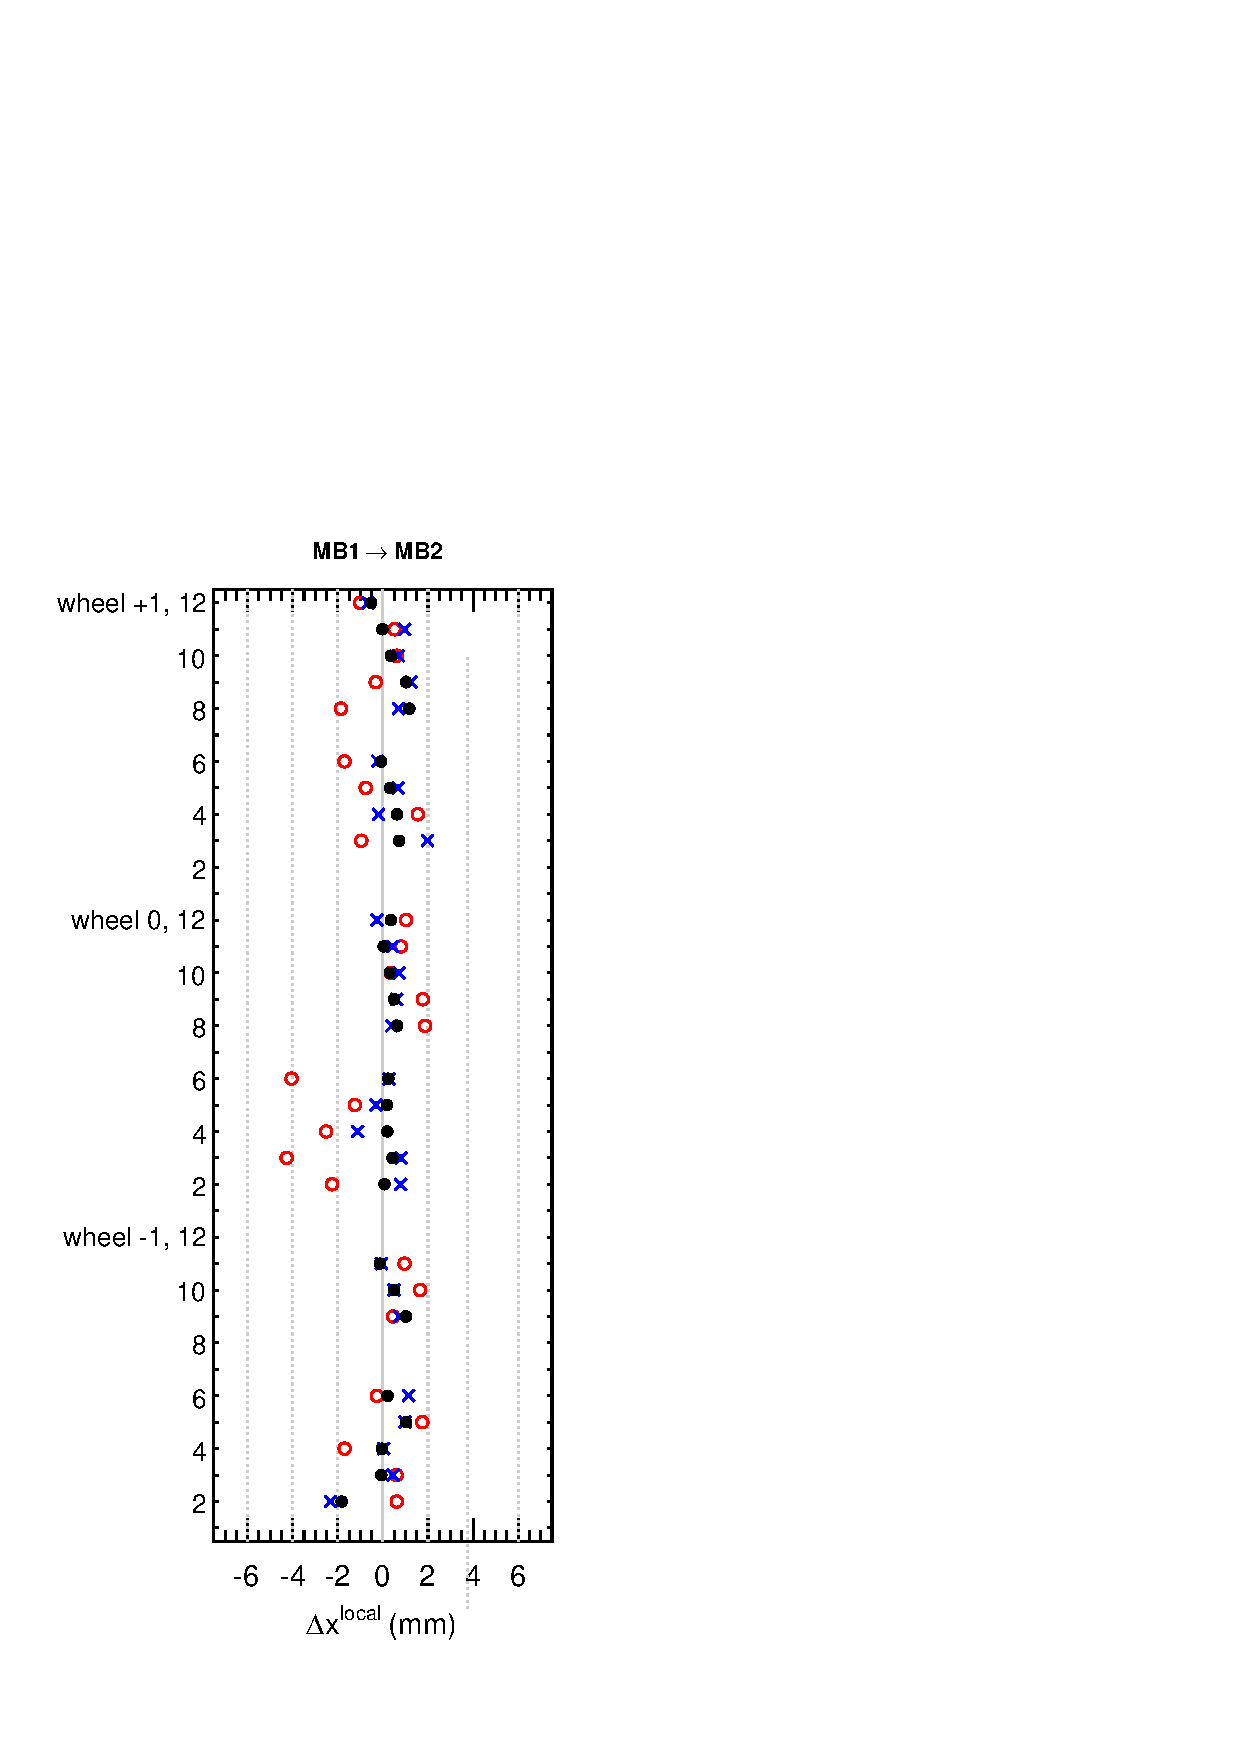
\includegraphics[width=0.32\linewidth]{plots/validation/segment_extrapolation_x12.pdf}
  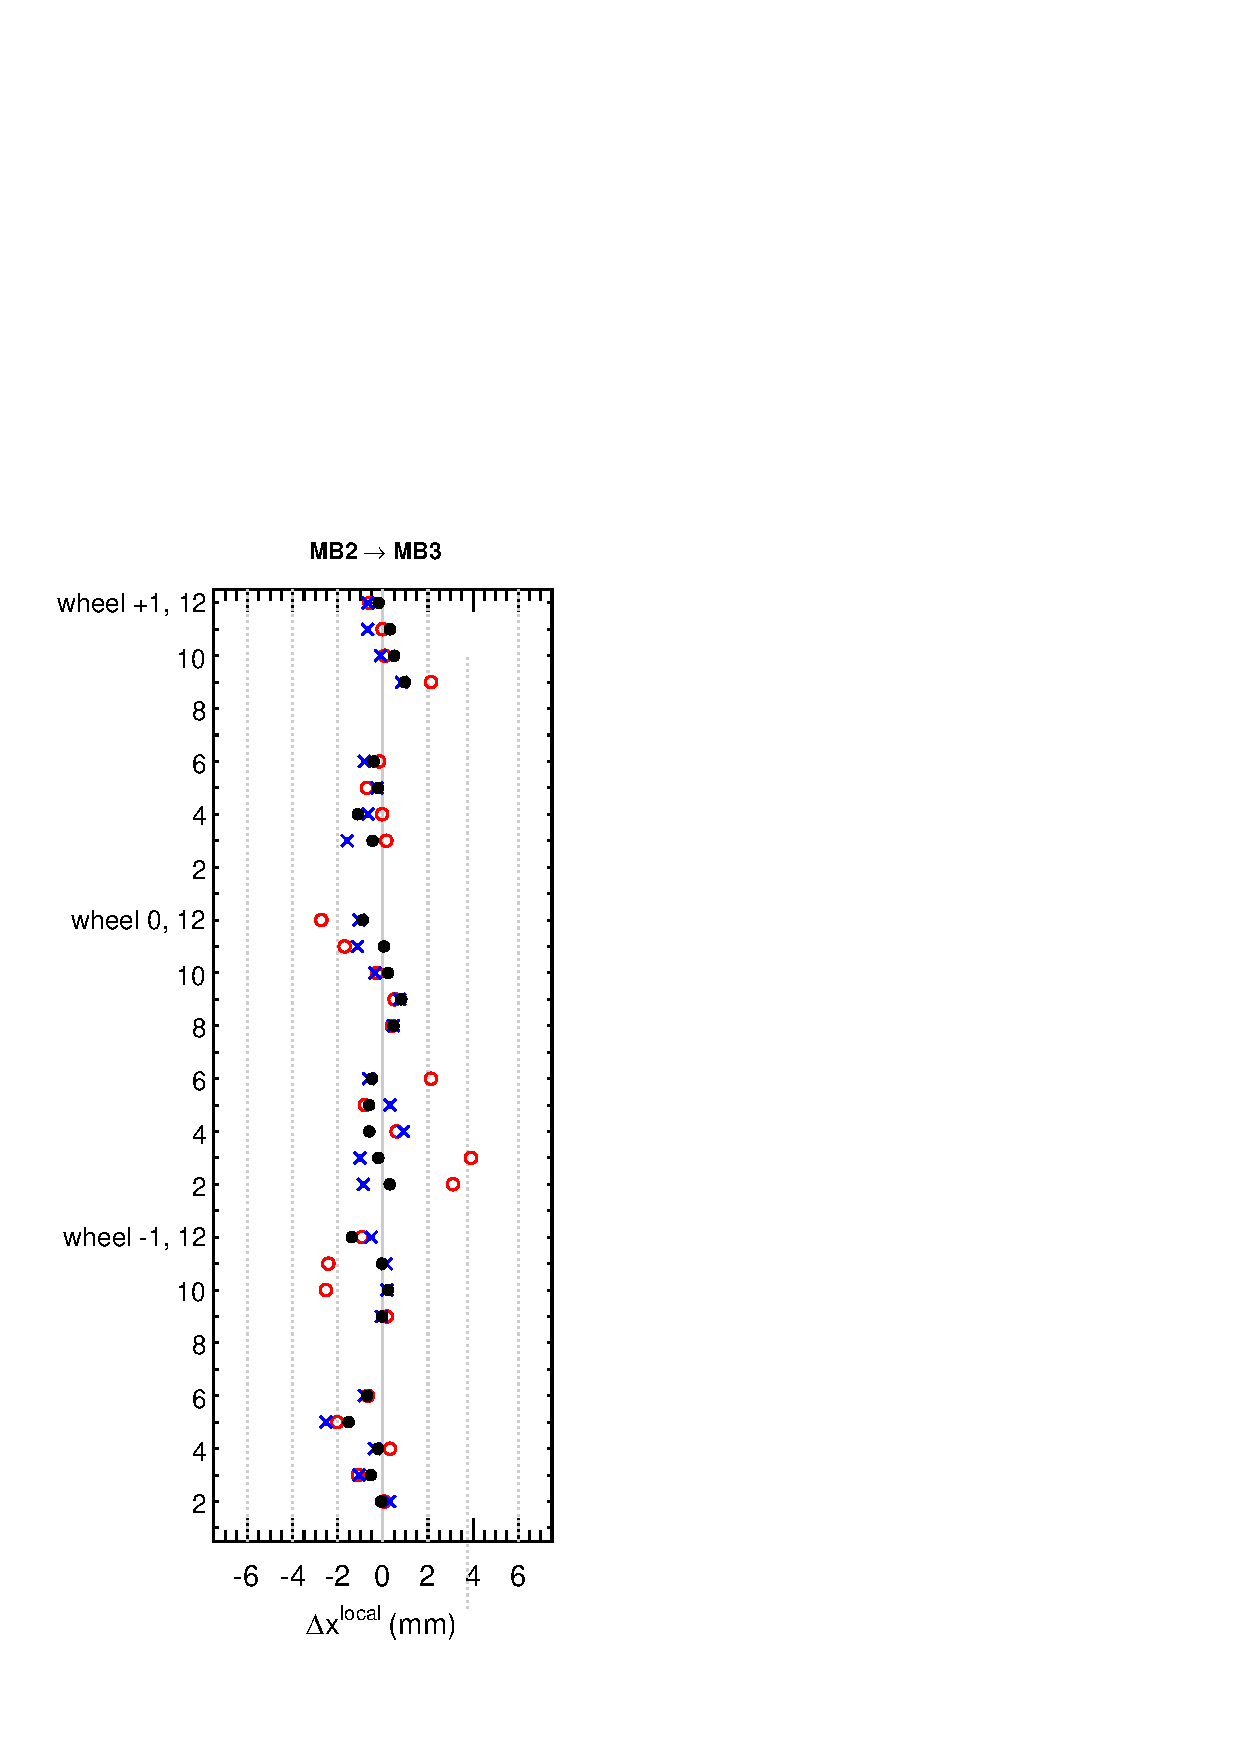
\includegraphics[width=0.32\linewidth]{plots/validation/segment_extrapolation_x23.pdf}
  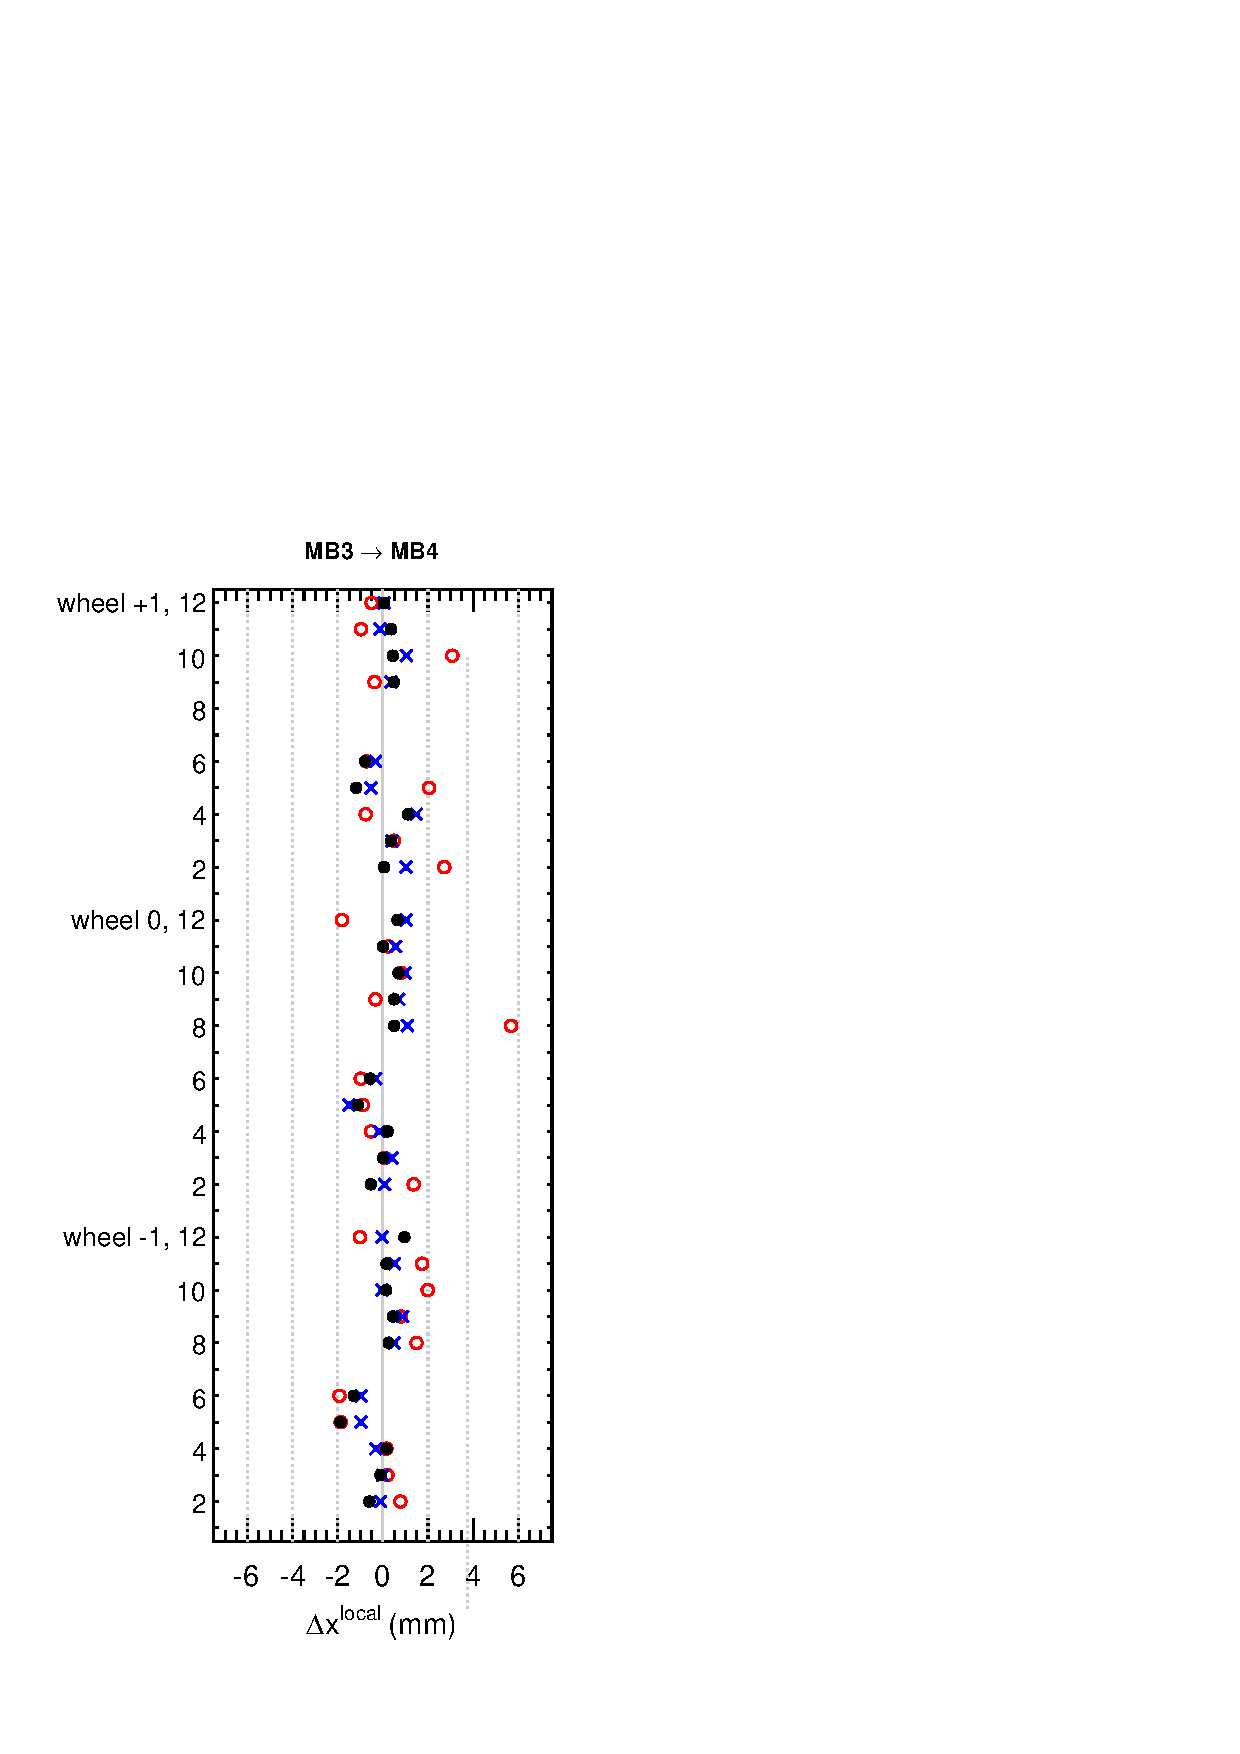
\includegraphics[width=0.32\linewidth]{plots/validation/segment_extrapolation_x34.pdf}

  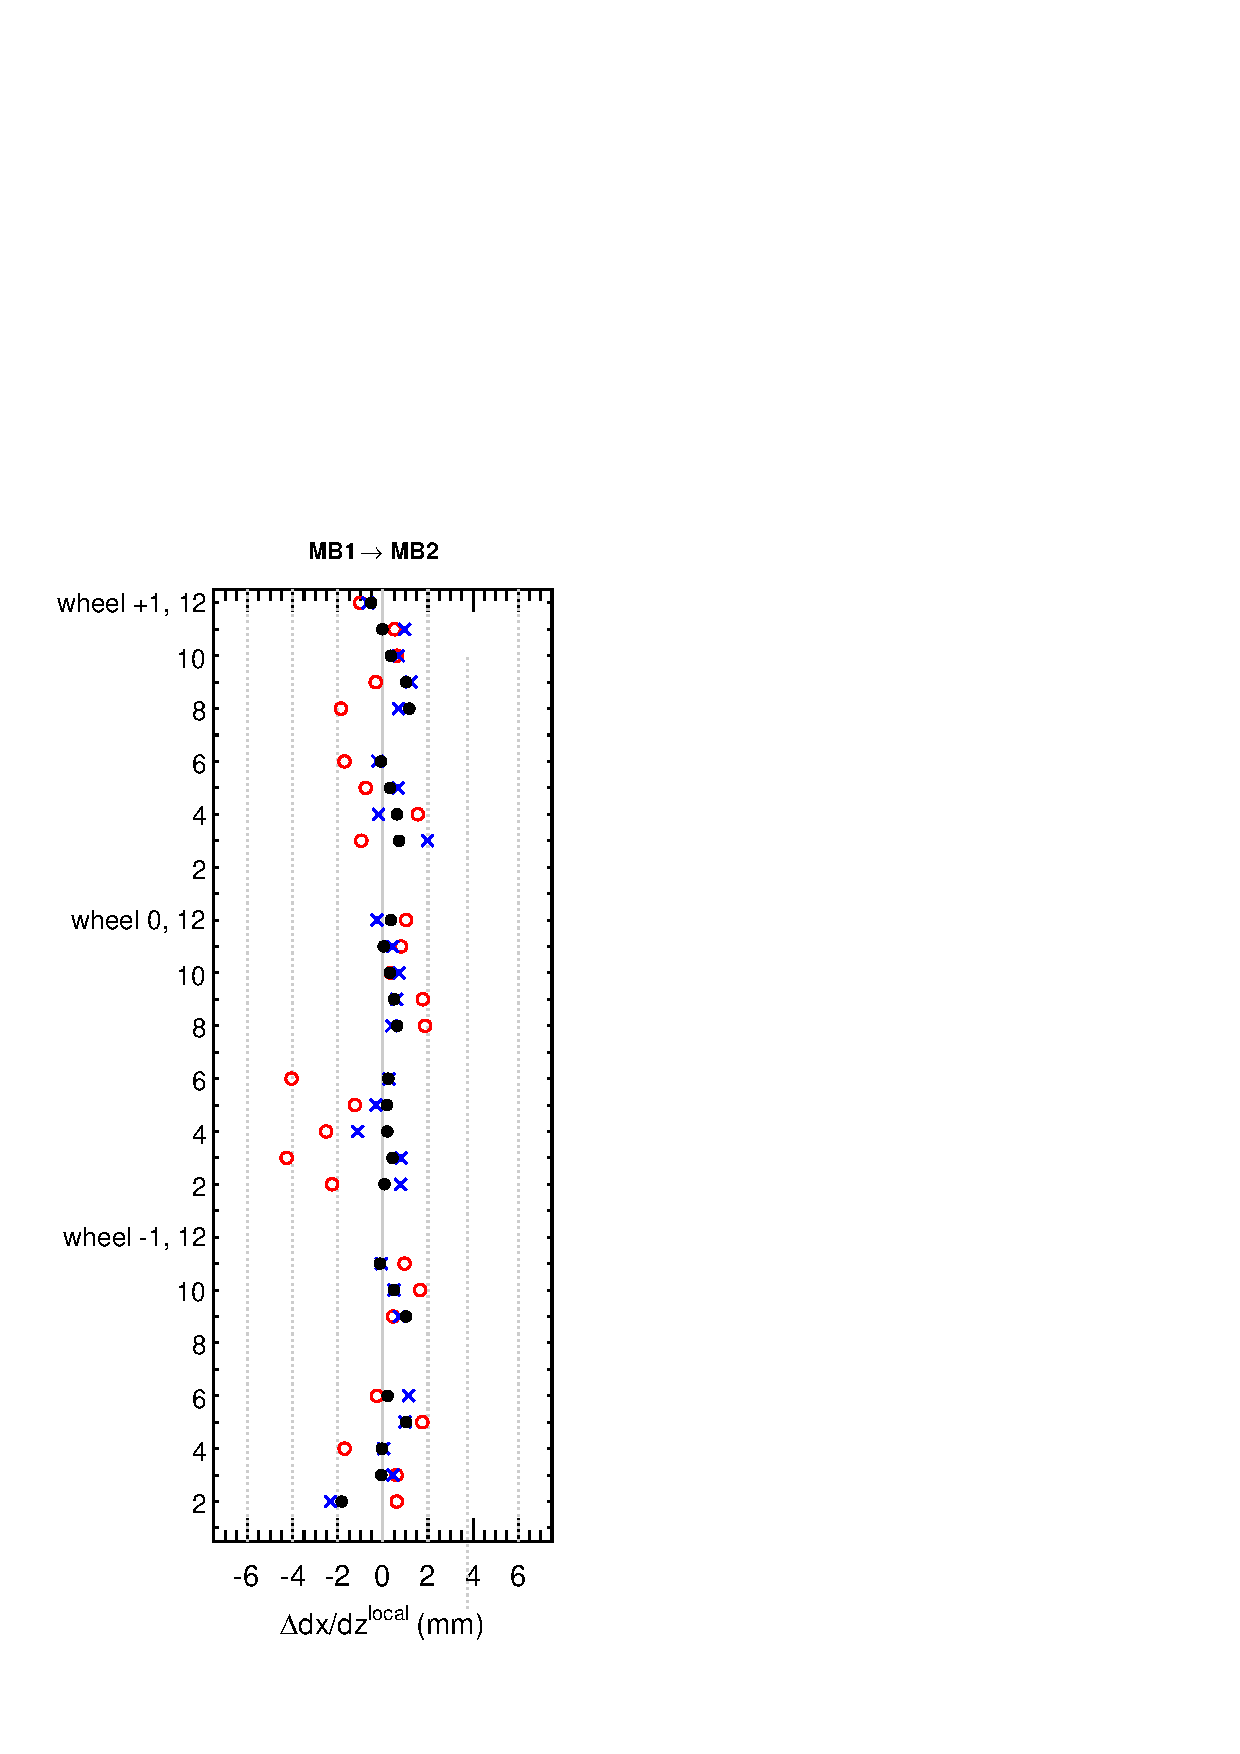
\includegraphics[width=0.32\linewidth]{plots/validation/segment_extrapolation_phi12.pdf}
  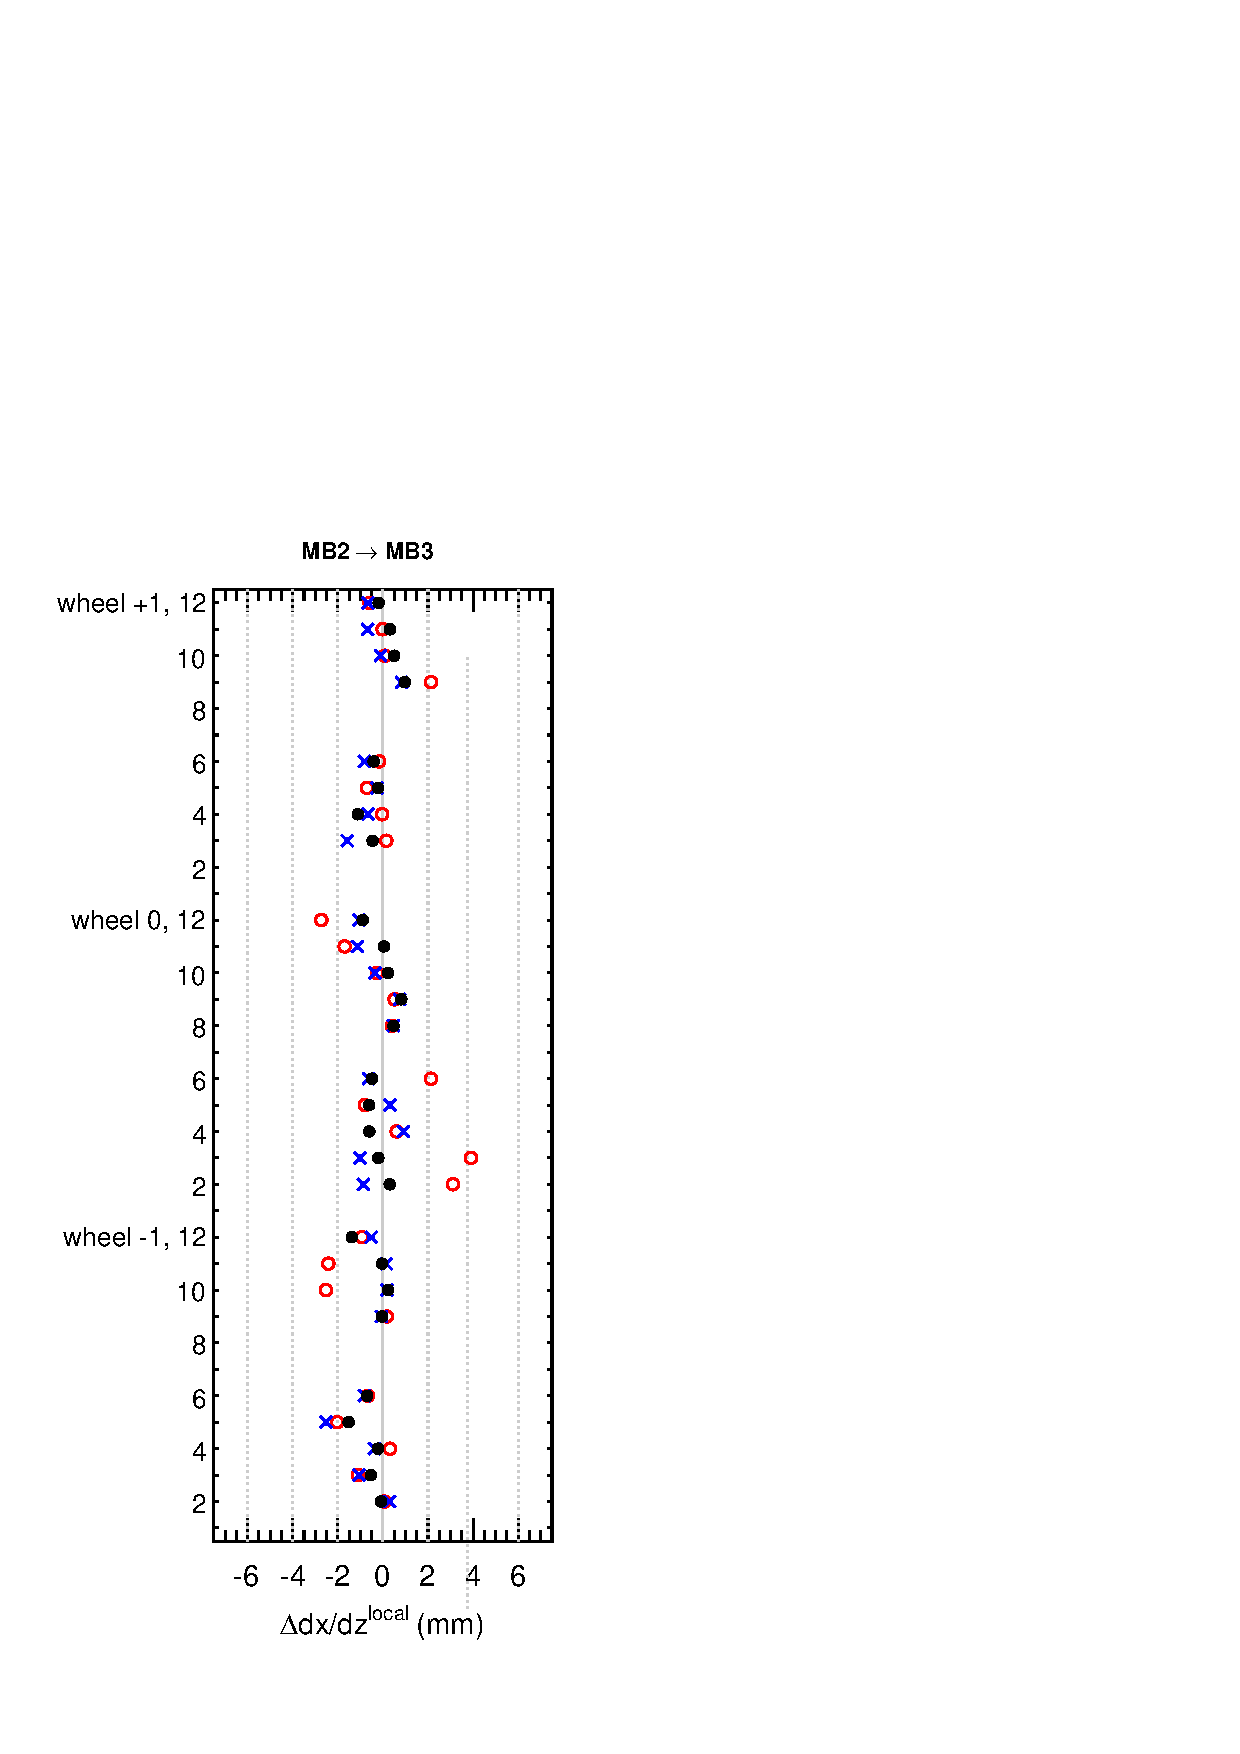
\includegraphics[width=0.32\linewidth]{plots/validation/segment_extrapolation_phi23.pdf}
  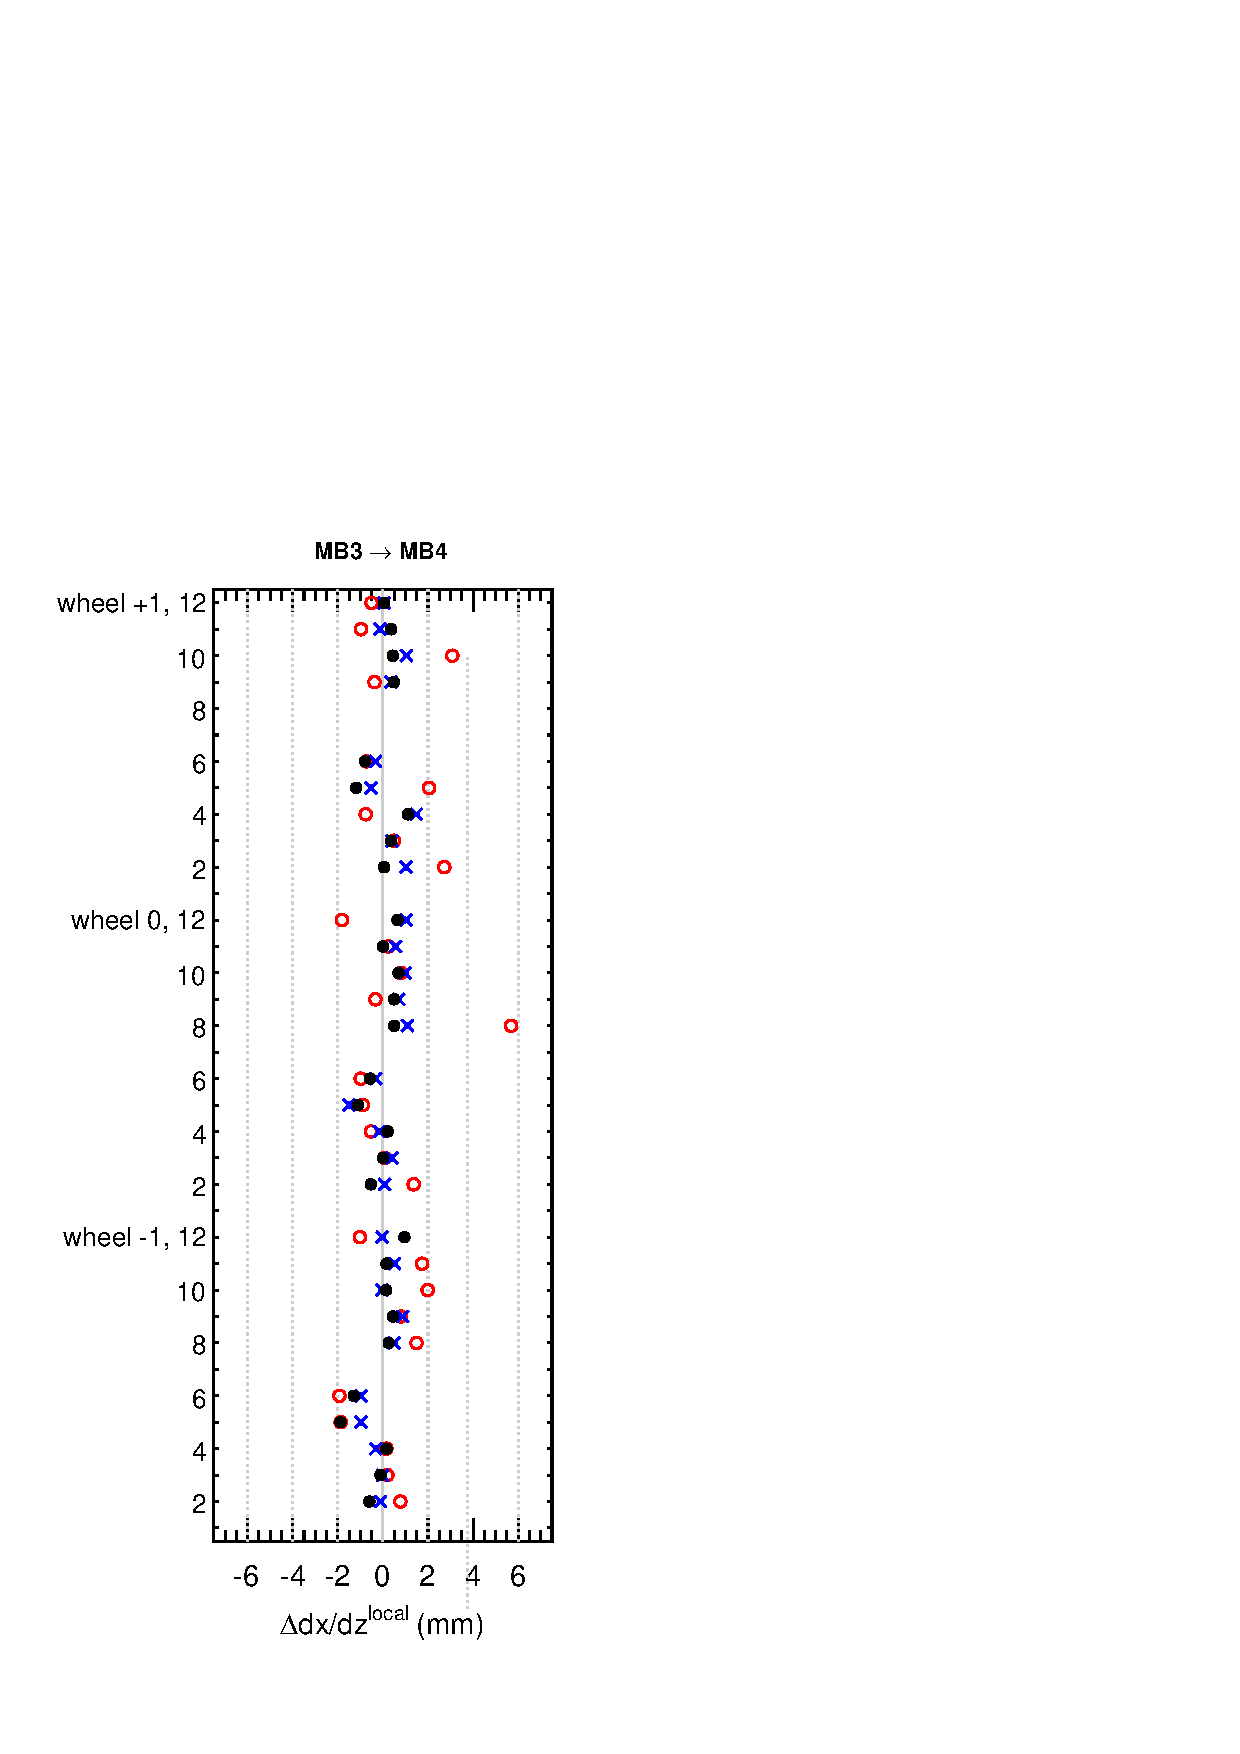
\includegraphics[width=0.32\linewidth]{plots/validation/segment_extrapolation_phi34.pdf}
  
  \caption{Local differences in alignment as measured by segments.
  The vertical axis labels wheel and sector numbers, and each plot
  shows one pair of stations for either local $x$ differences or
  $\phi_y$ differences, with different detector geometries. \label{fig:valid_NOMvsMPvsHIP}}
\end{figure}
 
To verify that the new alignment (in this case, HIP only) improves
momentum resolution (4), we selected cosmic rays with $p_T > 200$~GeV,
split each into two tracks near the origin (similar to what would be
observed in LHC collisions), and compared the momentum of the top and
bottom fits.  Since the cosmic ray muon is a single particle, any
mismatch between the halves is purely instrumental.  Cosmic rays have
a steeply falling distribution, so most of the selected tracks have
$p_T$ close to 200~GeV.  The alignment was performed using tracks with
$100 < p_T < 200$~GeV tracks, so the diagnostic sample is
statistically independent from the alignment.
Figure~\ref{fig:chargesplitting} compares tracker-only tracks and
tracks reconstructed with muon hits (first muon station only), before
and after the global muon alignment.

\begin{figure}
  \centering
  \subfigure{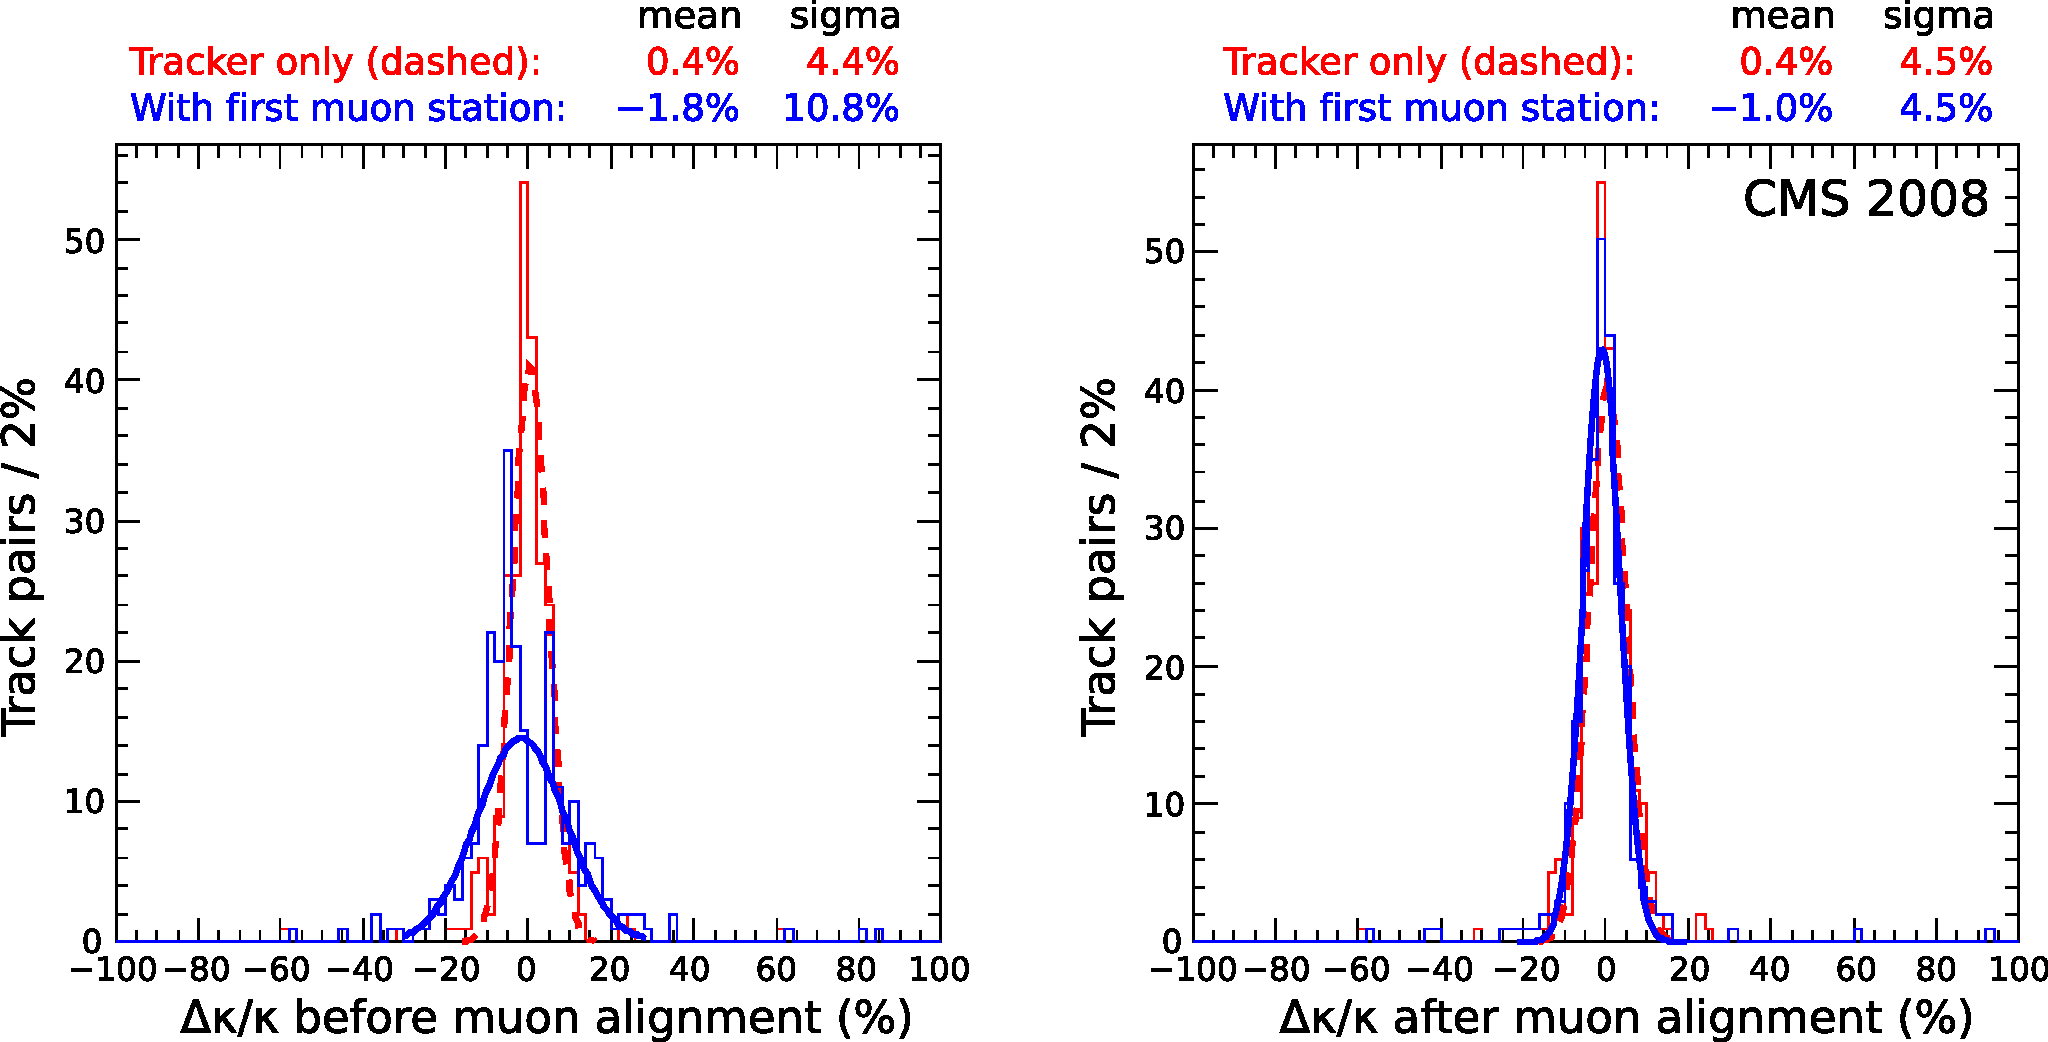
\includegraphics[width=\linewidth]{plots/monitoring_validation/chargesplitting_both.pdf}}
  \caption{Top vs.~bottom $1/p_T$ comparison for $p_T \gtrsim 200$~GeV split cosmic rays.\label{fig:chargesplitting}}
\end{figure}
